\section{LABORATORIOS CON SOFTWARE}
\begin{frame}

\pgfdeclareimage[width=\paperwidth,height=\paperheight]{bg}{imagenes/fondo_seccion}
\setbeamertemplate{background}{\pgfuseimage{bg}}

\definecolor{greenU}{RGB}{212,202,72}
\setbeamercolor{block body}{fg=Black,bg=greenU}
\begin{block}{}
\centering
\vspace{8mm}
\Large{LABORATORIOS CON SOFTWARE}
\vspace{8mm}
\end{block}
\end{frame}
%-----------------------

{
\begin{frame}
\frametitle{Parte I - Tabla de contenidos}
\begin{spacing}{1.5}
\tableofcontents[currentsection,sectionstyle=hide/hide,subsectionstyle=show/show/hide, subsubsectionstyle=hide]
\end{spacing}
\end{frame}
}

\subsection{Introducción a GNU Radio}

\begin{frame}{}

\pgfdeclareimage[width=\paperwidth,height=\paperheight]{bg}{imagenes/fondo_lab}
\setbeamertemplate{background}{\pgfuseimage{bg}}

\bfseries{\textrm{\Large \\Introducción a GNU Radio}}
\raggedright
\end{frame}



\begin{frame}
  
\pgfdeclareimage[width=\paperwidth,height=\paperheight]{bg}{imagenes/fondo3}
\setbeamertemplate{background}{\pgfuseimage{bg}}
  
  \frametitle{¿Qué es GNU Radio\index{GNU RADIO}?}

  
  Es una herramienta de desarrollo libre y abierta que provee bloques de procesamiento de señal para implementar sistemas de radio definido por software. Puede utilizarse con hardware de RF para crear radios definidos por
software o sin hardware para crear un ambiente de simulación. Es utilizada
extensivamente en ambientes académicos, aficionados y comerciales para dar
soporte a la investigación en comunicaciones inalámbricas y en sistemas de
radio en el mundo.
\end{frame}



\begin{frame}{Aplicaciones\index{Aplicaciones}}
  \begin{figure}[H]
  \centering
  \includegraphics[width=0.9\textwidth]{parte1/intro/pdf/intro.pdf}
  \end{figure}
  
  
\end{frame}



\begin{frame}{Instalación de GNU Radio en Linux}
{Para instalar GNU Radio se deben seguir los siguientes pasos:}
\begin{enumerate}[1.]
\item Ingresar a la ventana de órdenes (o terminal) del sistema de su equipo.
\item Estando conectado a internet, escriba dentro del terminal:

  \begin{block}{}
  \texttt{ sudo apt-get install gnuradio}
  \end{block}

\item Si su dispositivo tiene contrase\~na, debe ingresarla, al ser solicitada y oprimir \keys{\return}. 
\item Luego se deben aceptar los términos de la instalación oprimiendo la letra \keys{s} seguido de \keys{\return}. 
\item Una forma de verificar la correcta instalación es volviendo a ingresar la orden indicada en el punto 2, y si aparece un mensaje anunciando que GNU Radio ya está en su versión más reciente, su instalación fue correcta.
\end{enumerate}
\end{frame}
%----------------------------

\begin{frame}{Paquetes\index{Paquetes}}
Con el objetivo de clonar el repositorio y obtener los ejemplos de GNU Radio en nuestro ordenador se deben instalar los siguientes paquetes: 
  \begin{itemize}
  \item {\tt build-essential}

    Build essential es un paquete que contiene herramientas necesarias
    para la creación, compilación e instalación de programas.
  
  \item {\tt cmake}

  Es un sistema de construcción de código abierto multiplataforma. Se trata de
un conjunto de herramientas diseñadas para construir, testear y empaquetar
software. Se utiliza para controlar el proceso de compilación de software
utilizando una plataforma sencilla y unos archivos de configuración
independientes del compilador.

  \end{itemize}

\end{frame}
%-------------------------------

\begin{frame}{Paquetes}
  \begin{itemize}
  \item {\tt git}

    Este paquete contiene un sistema de control de versiones
distribuidas de código abierto desarrollado originalmente por Linux Torvalds
para apoyar el desarrollo del kernel de Linux.
    
	El control de versiones es un sistema que registra los cambios
realizados sobre un archivo o conjunto de archivos a lo largo del tiempo, de
modo que se puedan recuperar versiones específicas más adelante.
  
	\item {\tt libboost-all-dev} 
  
	Boost es un conjunto de bibliotecas para el lenguaje de programación
C++ que suministra un apoyo para tareas y estructuras como álgebra lineal,
generación de números pseudoaleatorios, procesamiento de imágenes, expresiones
regulares y pruebas unitarias. En el momento contiene 162 bibliotecas
individuales.
  
	\end{itemize}
\end{frame}

%++++++++++++++++++++

\begin{frame}{Paquetes\index{Paquetes}}
  \begin{itemize}
  \item {\tt libcppunit-dev}
  \begin{itemize}
    \item
    {Biblioteca de pruebas unitarias para C++.}
    \item
    {Una prueba unitaria es una forma de comprobar el correcto
funcionamiento de una unidad de código. Por ejemplo, en diseño
estructurado o en diseño funcional, una función o un procedimiento,
en diseño orientado a objetos una clase. Esto sirve para asegurar que
cada unidad funcione correcta y eficientemente por separado.}
    \end{itemize}
  \item {\tt doxygen}
  {Es una herramienta para generar documentación a partir de código fuente. Es un sistema de documentación para C++, C, Java, Python. Es necesario solo si se desea generar referencias a documentación externa de la que no tiene las fuentes.}
  \end{itemize}
\end{frame}

%+++++++++++++++++++

\begin{frame}{Instalación de paquetes}
\begin{enumerate}[1.]
\item La instalación de cada uno se los paquetes anteriormente mencionados se realiza colocando en la ventana de terminal, las siguientes órdenes:
\end{enumerate}

  \begin{block}{}
  \texttt{
  \ \ \ sudo apt-get install build-essential
    \begin{itemize}
      \item[] sudo apt-get install cmake
      \item[] sudo apt-get install git
      \item[] sudo apt-get install libboost-all-dev
      \item[] sudo apt-get install libcppunit-dev
      \item[] sudo apt-get install doxygen
    \end{itemize}}
  \end{block}


\end{frame}

%++++++++++++++++++++


\begin{frame}{Clonar repositorio\index{Clonar Repositorio}}
El código fuente de los ejemplos está almacenado en github, por lo tanto para clonar el repositorio se debe realizar lo siguiente:
\begin{itemize}
\item Abrir la ventana de órdenes o terminal.
\item Después se debe ingresar la siguiente orden para clonar el directorio git:

\begin{block}{}
  \texttt{
    git clone https://github.com/gnuradio/gr-tutorial}
  \end{block}

\item Una vez clonado el directorio, {\tt gr-tutorial}, en el PC empleado se deben ver exactamente los mismos archivos y carpetas que los del repositorio github.
\end{itemize}
\end{frame}

%+++++++++++++++++++

\begin{frame}{Instalación de módulos\index{Modulos}}
\begin{itemize}
\item Luego de haber clonado el repositorio, debemos buscar la carpeta \textbf{“gr-tutorial”} e ingresar a ella desde el terminal, para ello se digitan las siguientes órdenes:

  \begin{block}{}
  \texttt{
  \ \ \ ls
    \begin{itemize}
      \item[] cd gr-tutorial
    \end{itemize}}
  \end{block}

Es importante mencionar que al escribir la primera orden se podrán observar la diferentes carpetas que se encuentran en el dispositivo, por lo tanto \textbf{“gr-tutorial”} debe aparecer entre las opciones para poder cambiar de directorio. 
\end{itemize}
\end{frame}

%+++++++++++++++

\begin{frame}{Instalación de módulos\index{Modulos}}
\begin{itemize}
\item Estando dentro de la carpeta, desde la terminal, se deben escribir las siguientes órdenes, con la finalidad de instalar las soluciones o módulos:

  \begin{block}{}
  \texttt{
  \ \ \ mkdir build
    \begin{itemize}
      \item[] cd build
      \item[] cmake ..
      \item[] make -j8
      \item[] sudo make install
      \item[]sudo ldconfig
    \end{itemize}}
  \end{block}

\end{itemize}
\end{frame}

\begin{frame}{Resultado}
En el directorio {\tt examples} encontrará los tutoriales:
  \begin{block}{}
  \texttt{
    \begin{itemize}
      \item[] tutorial1
      \item[] tutorial2
      \item[] ...
      \item[] tutorial7
    \end{itemize}}
  \end{block}

Puede explorar los ejemplos de los desarrolladores de GNU Radio 
\end{frame}


%///////////////////////////////////////////////////////////////
\subsection{Lab6: Interfaces gráficas de  WX GUI}
%*********************
\begin{frame}{}

\pgfdeclareimage[width=\paperwidth,height=\paperheight]{bg}{imagenes/fondo_lab}
\setbeamertemplate{background}{\pgfuseimage{bg}}

\bfseries{\textrm{\LARGE Interfaces gráficas con \newline WX GUI}}
\raggedright
\end{frame}
%*********************

\begin{frame}{Grid position}

\pgfdeclareimage[width=\paperwidth,height=\paperheight]{bg}{imagenes/fondo3}
\setbeamertemplate{background}{\pgfuseimage{bg}}

\textbf {Posicionamiento de rejilla} \\
\vspace{2mm}
GRC ofrece varios receptores gráficos y controles gráficos para crear gráficos de flujo wx-gui.(scope sink, fft sink, number sink, waterfall sink, constellation sink, slider control, and chooser control) Cada uno de estos elementos gráficos tiene un parámetro de posición de cuadrícula para un posicionamiento preciso.

\end{frame}
%-----------------------------------

\begin{frame}{Grid position}

\begin{figure}[H]
\centering
\vspace{-3mm}
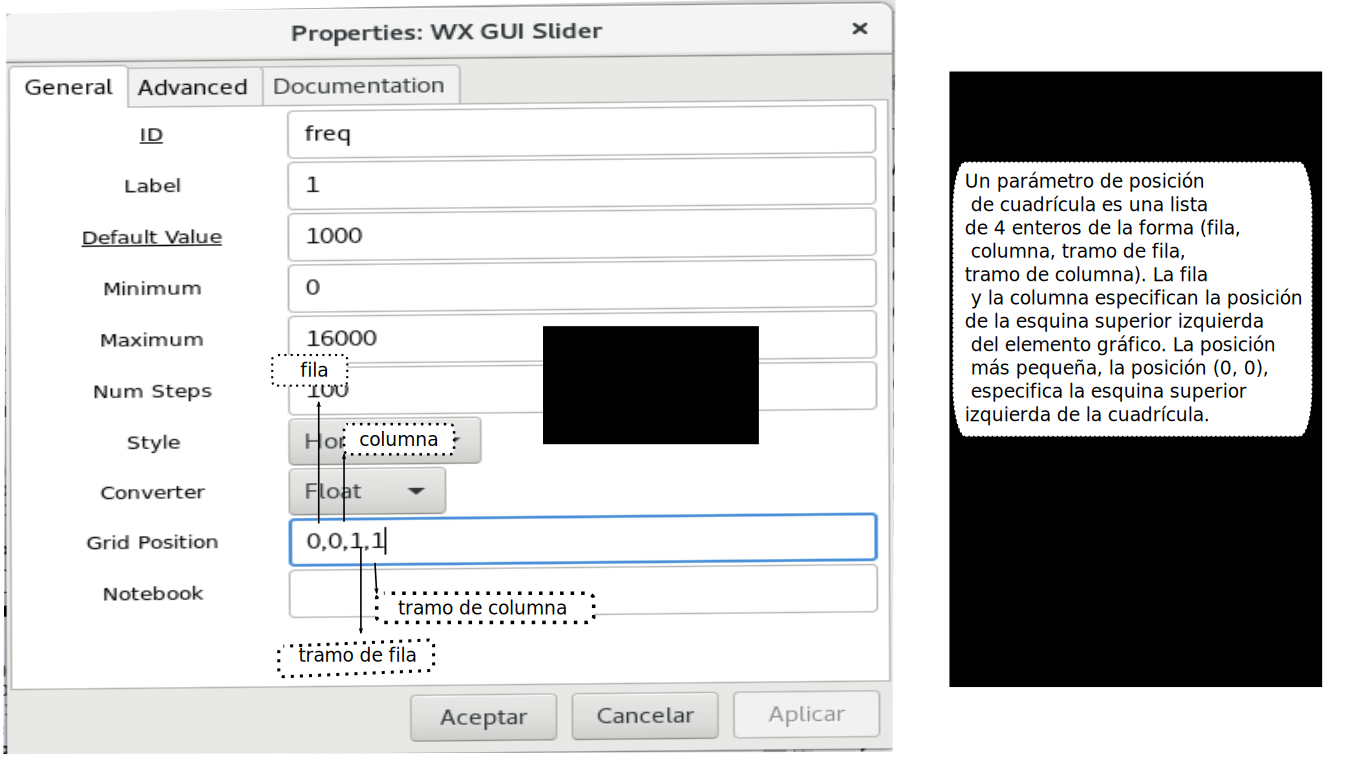
\includegraphics[width=0.9\textwidth]{parte1/lab00/pdf/lab0_1.pdf}


\end{figure}

\end{frame}
%-----------------------------------

\begin{frame}{Grid position}

El tramo de fila especifica el número de filas hacia abajo desde la posición de la fila, y el tramo de columna especifica el número de columnas a la derecha de la posición de la columna. Por lo tanto, el tramo debe ser al menos (1, 1) para ocupar el mínimo de 1 celda de cuadrícula.

\end{frame}
%-----------------------------------

\begin{frame}{Grid position}

\begin{figure}[H]
\centering
\vspace{-3mm}
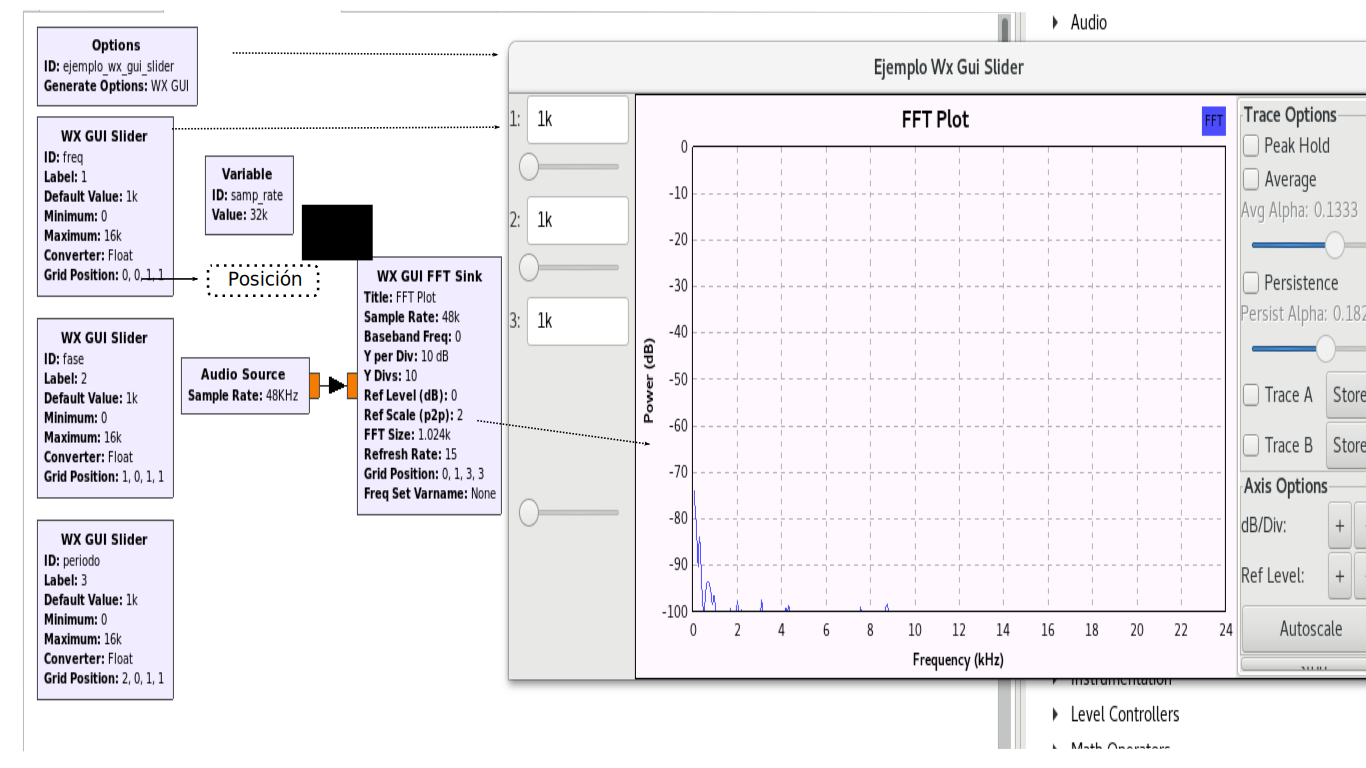
\includegraphics[width=0.9\textwidth]{parte1/lab00/pdf/lab0_2.pdf}
\end{figure}

\end{frame}
%-----------------------------------

\begin{frame}{Grid position}

\begin{figure}[H]
\centering
\vspace{-3mm}
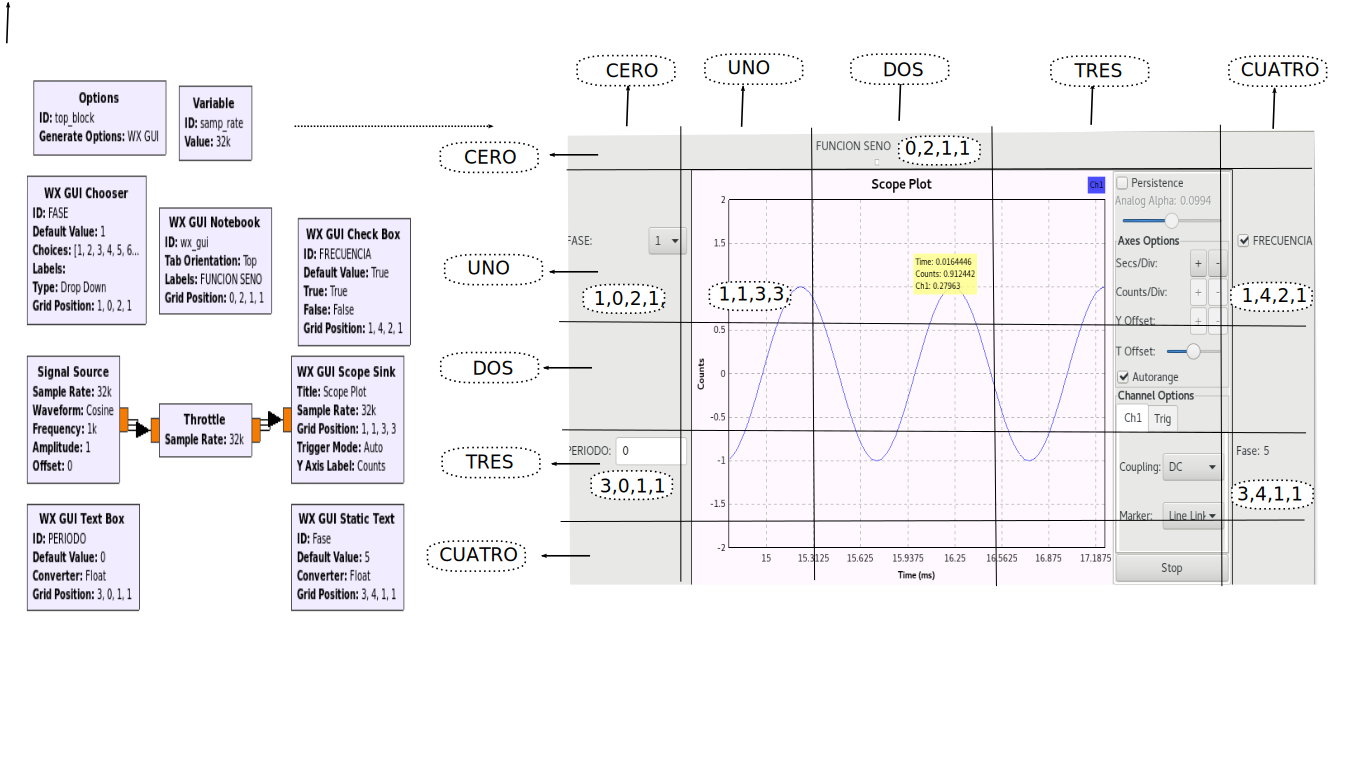
\includegraphics[width=0.9\textwidth]{parte1/lab00/pdf/lab0_3.pdf}
\end{figure}

\end{frame}
%-----------------------------------


%///////////////////////////////////////////////////////////////
\subsection{Lab1: Primeros pasos}
%*********************
\begin{frame}{}

\pgfdeclareimage[width=\paperwidth,height=\paperheight]{bg}{imagenes/fondo_lab}
\setbeamertemplate{background}{\pgfuseimage{bg}}

\bfseries{\textrm{\LARGE Lab1\\ \Large Primeros pasos}}
\raggedright
\end{frame}
%*********************

\begin{frame}{Primeros pasos}

\pgfdeclareimage[width=\paperwidth,height=\paperheight]{bg}{imagenes/fondo3}
\setbeamertemplate{background}{\pgfuseimage{bg}}

\begin{figure}[H]
\centering
\vspace{-3mm}
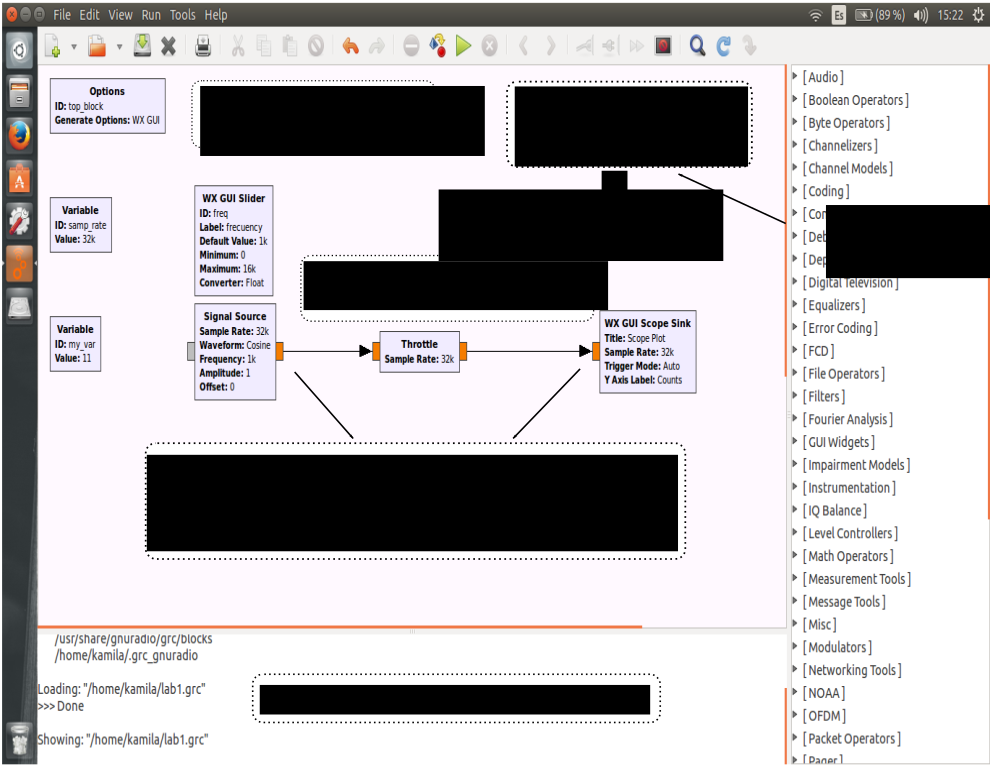
\includegraphics[width=0.9\textwidth]{parte1/lab1/pdf/lab1_1.pdf}
\end{figure}
\end{frame}
%-----------------------------------

\begin{frame}{Primeros pasos }
\begin{figure}[H]
\centering
\vspace{-3mm}
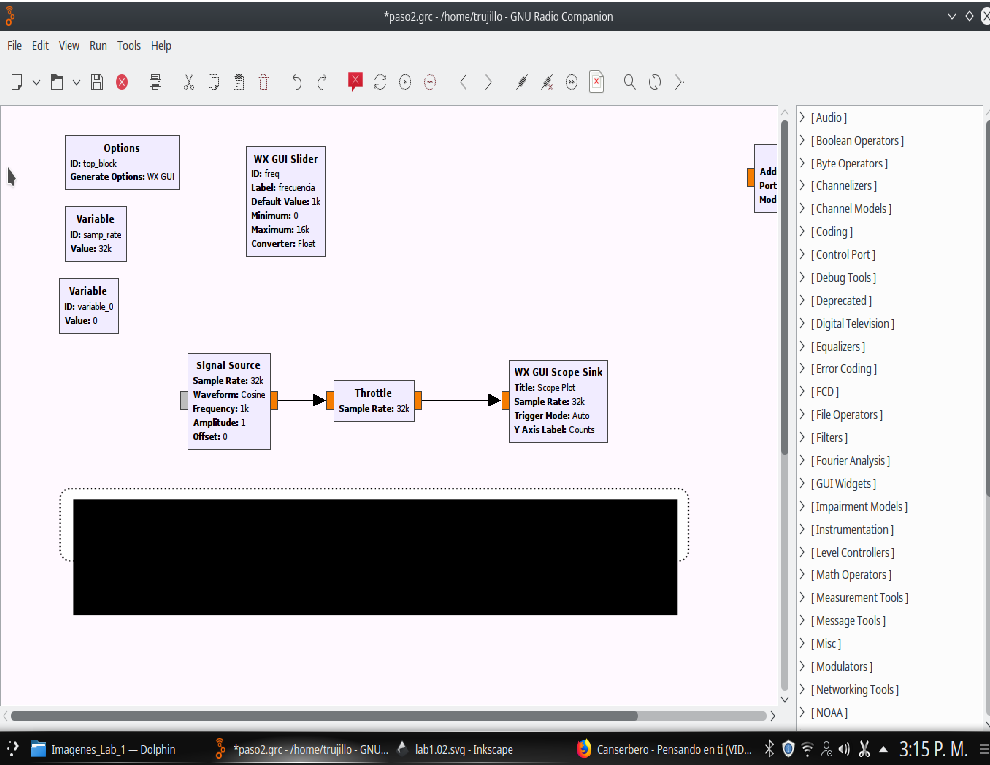
\includegraphics[width=0.9\textwidth]{parte1/lab1/pdf/lab1_2.pdf}
\end{figure}
\end{frame}
%-----------------------------------

\begin{frame}{Primeros pasos }
\begin{figure}[H]
\vspace{-3mm}
\centering
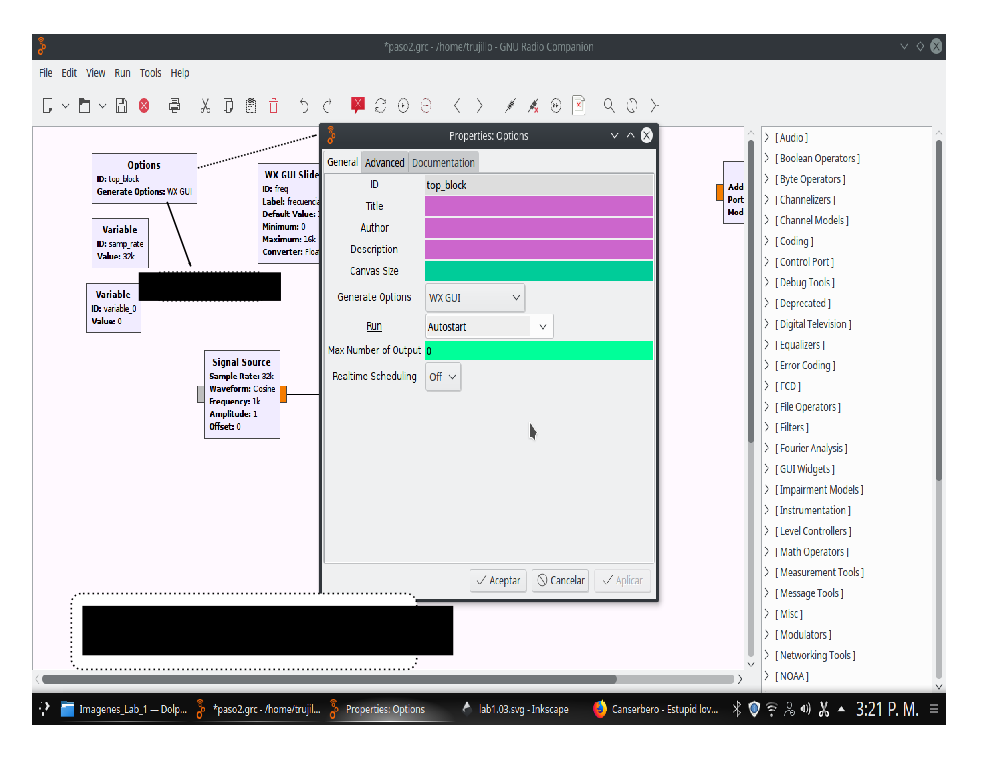
\includegraphics[width=0.9\textwidth]{parte1/lab1/pdf/lab1_3.pdf}
\end{figure}
\end{frame}
%-----------------------------------

\begin{frame}{Primeros pasos }
\begin{figure}[H]
\vspace{-3mm}
\centering
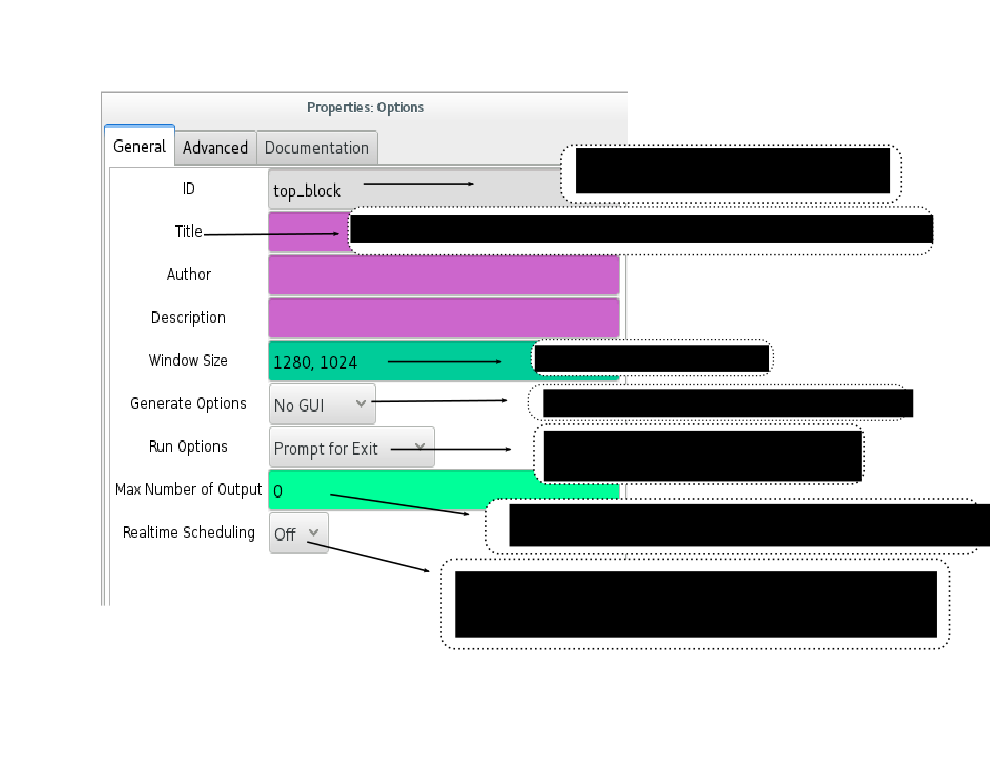
\includegraphics[width=0.9\textwidth]{parte1/lab1/pdf/lab1_4.pdf}
\end{figure}
\end{frame}
%-----------------------------------

\begin{frame}{Primeros pasos }
\begin{figure}[H]
\vspace{-2cm}
\centering
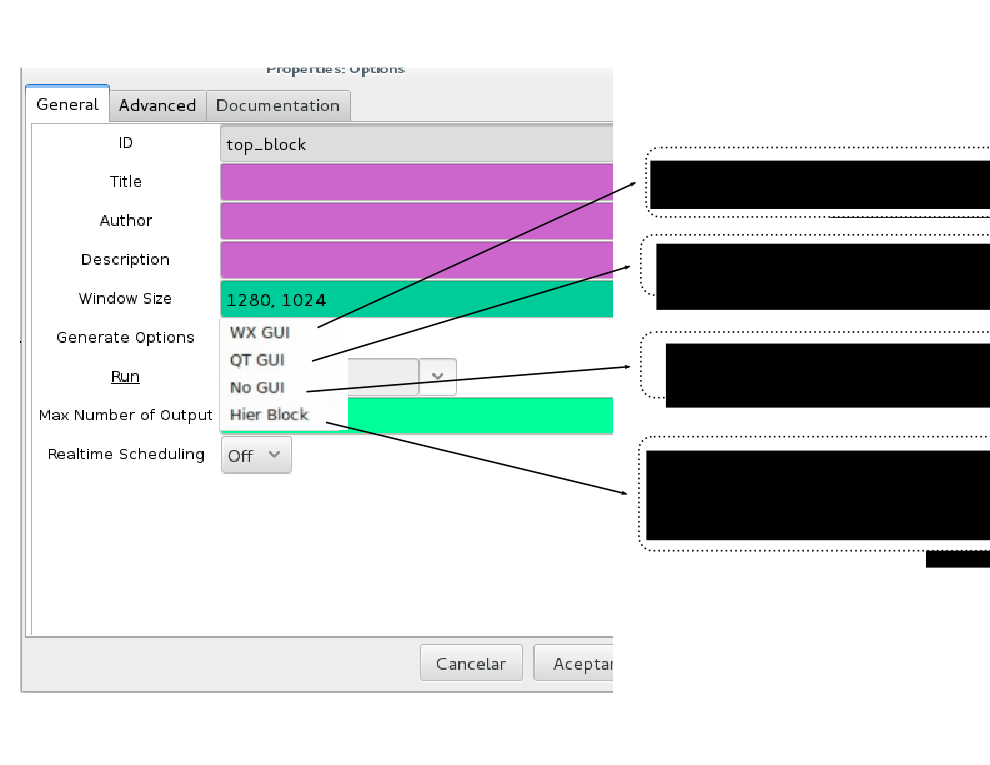
\includegraphics[width=1.1\textwidth]{parte1/lab1/pdf/lab1_5.pdf}
\end{figure}
\end{frame}
%-----------------------------------

\begin{frame}{Primeros pasos }
\begin{figure}[H]
\centering
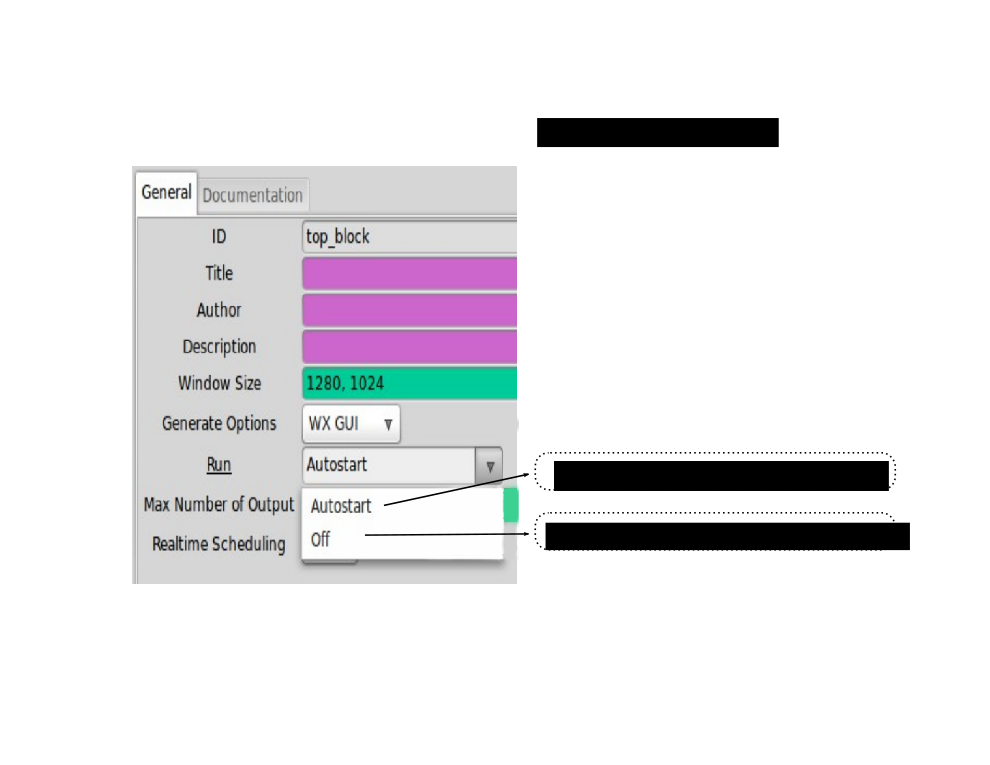
\includegraphics[width=.9\textwidth]{parte1/lab1/pdf/lab1_6.pdf}
\end{figure}
\end{frame}
%-----------------------------------

\begin{frame}{Primeros pasos }
\begin{figure}[H]
\centering
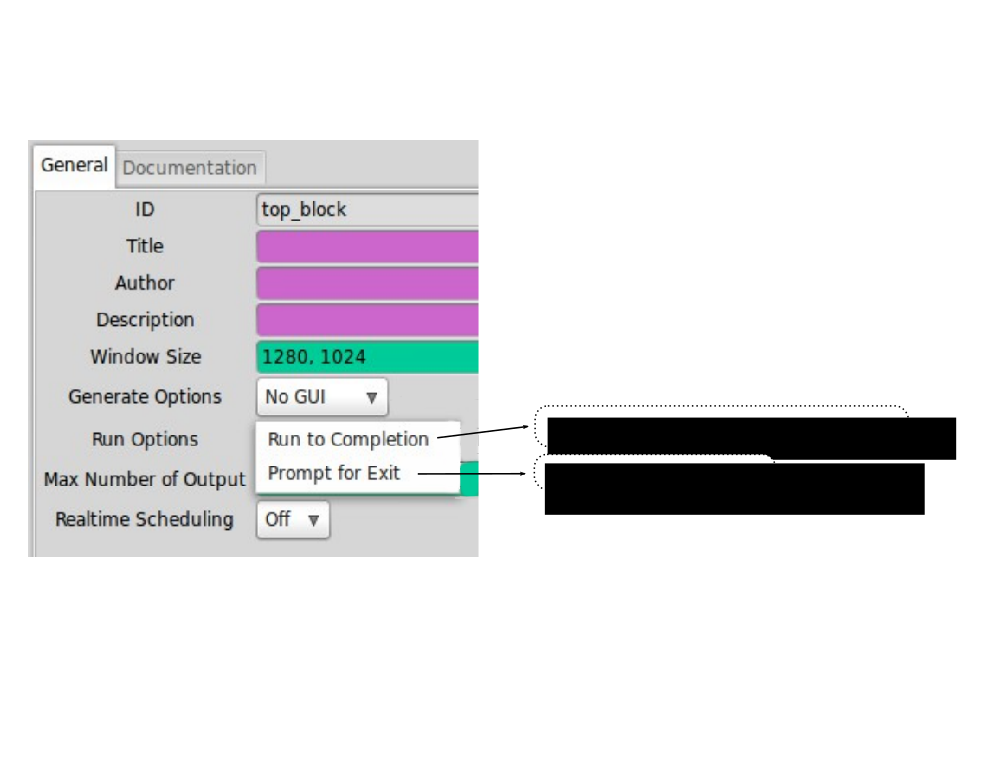
\includegraphics[width=\textwidth]{parte1/lab1/pdf/lab1_7.pdf}
\end{figure}
\end{frame}
%-----------------------------------

\begin{frame}{Primeros pasos }
\begin{figure}[H]
\vspace{-1cm}
\centering
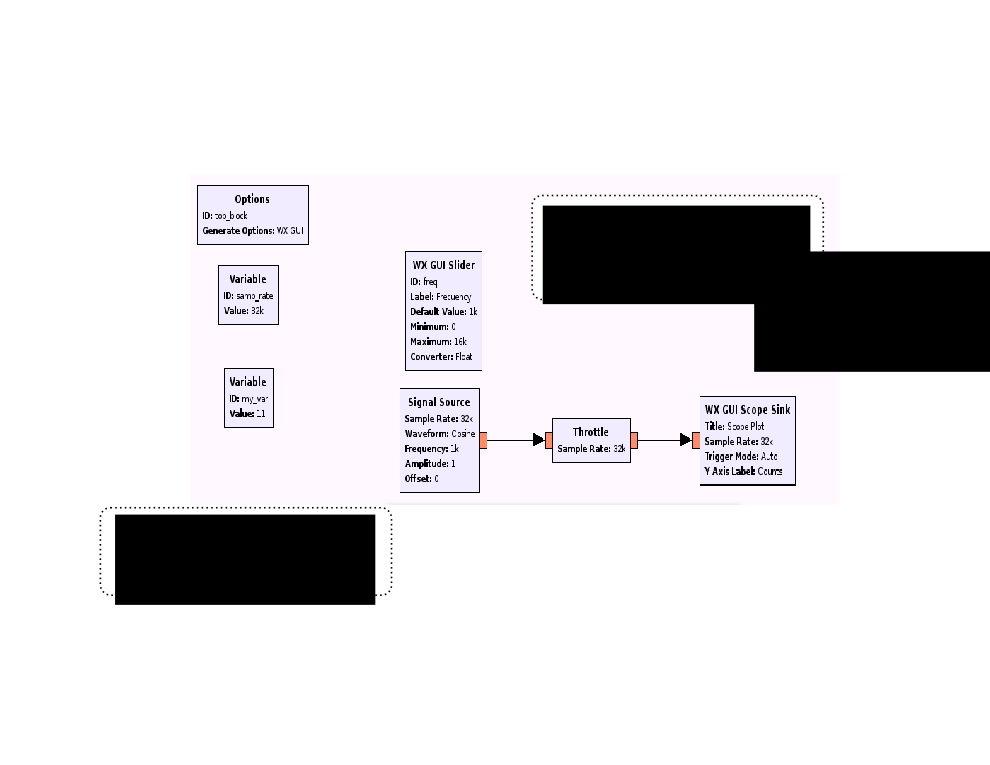
\includegraphics[width=\textwidth]{parte1/lab1/pdf/lab1_8.pdf}
\end{figure}
\end{frame}
%-----------------------------------

\begin{frame}{Primeros pasos }
\begin{figure}[H]
\vspace{-3mm}
\centering
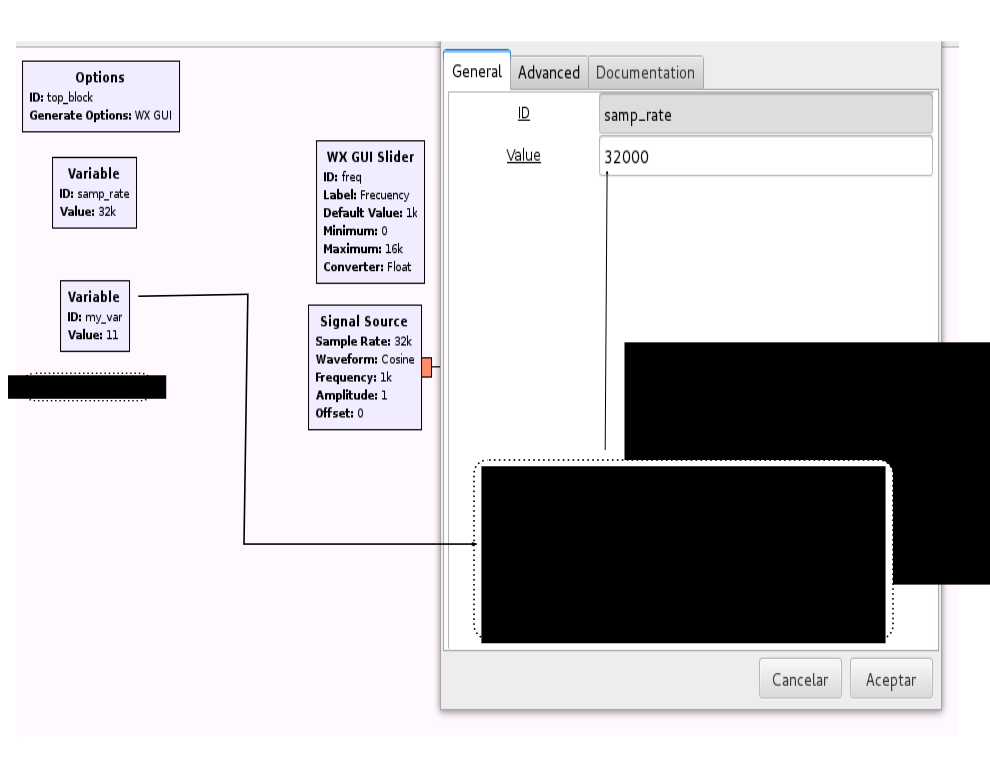
\includegraphics[width=0.85\textwidth]{parte1/lab1/pdf/lab1_9.pdf}
\end{figure}
\end{frame}
%-----------------------------------

\begin{frame}{Primeros pasos }
\begin{figure}[H]
\vspace{-3mm}
\centering
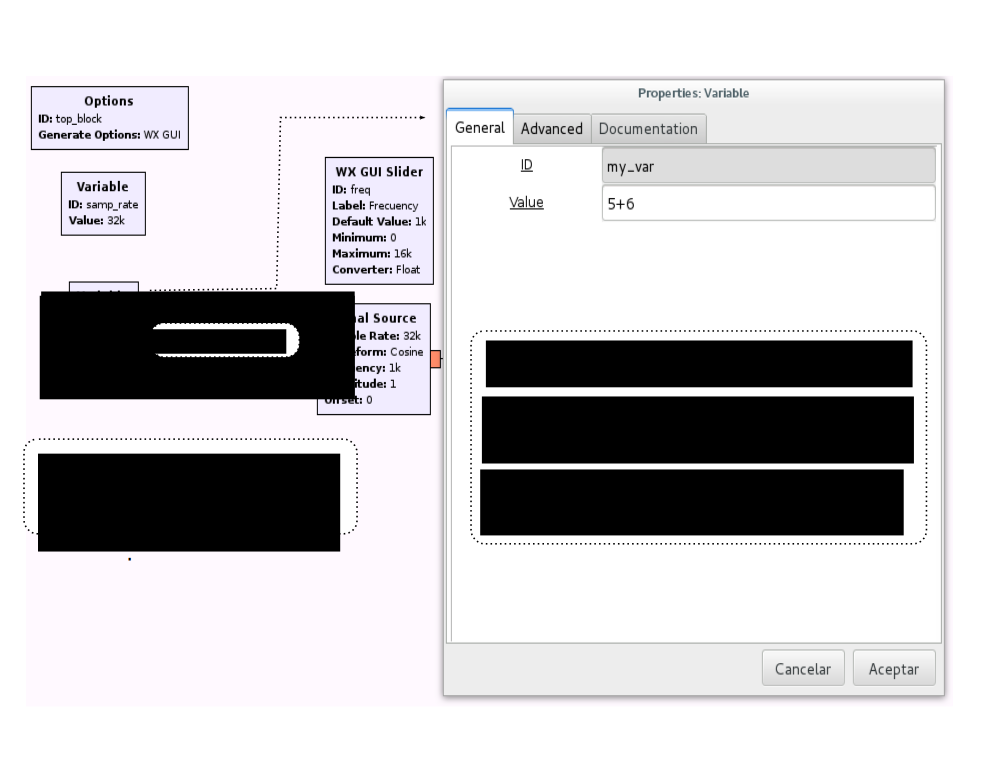
\includegraphics[width=.9\textwidth]{parte1/lab1/pdf/lab1_10.pdf}
\end{figure}
\end{frame}
%-----------------------------------

\begin{frame}{Primeros pasos }
\begin{figure}[H]
\vspace{-3mm}
\centering
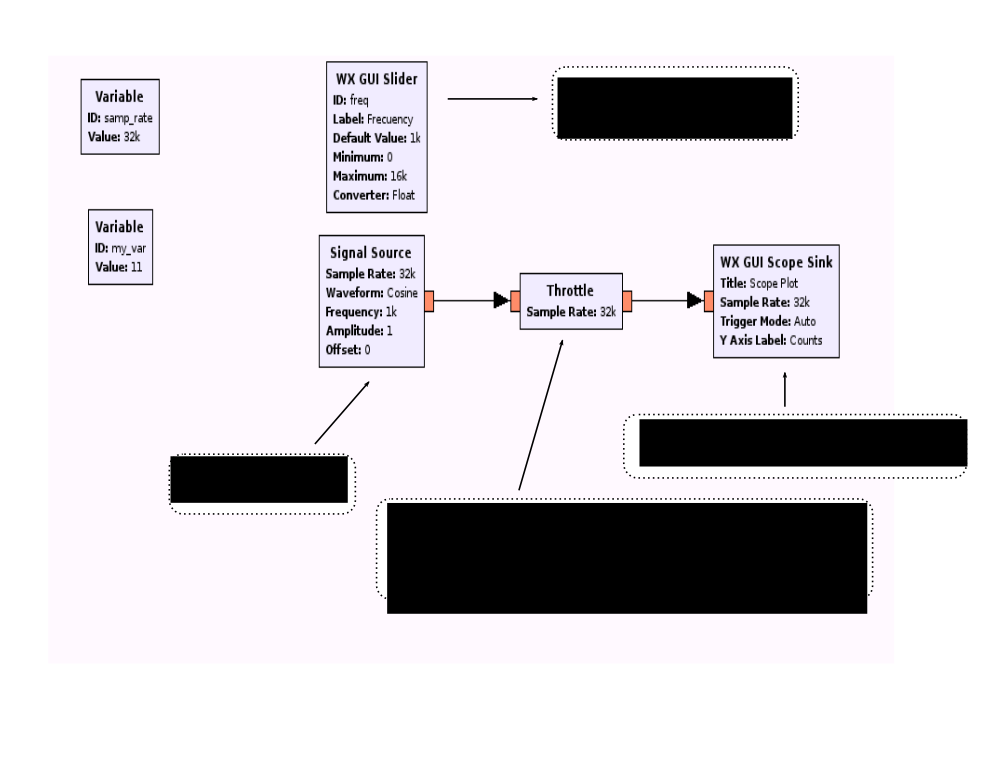
\includegraphics[width=\textwidth]{parte1/lab1/pdf/lab1_11.pdf}
\end{figure}
\end{frame}
%-----------------------------------

\begin{frame}{Primeros pasos }
\begin{figure}[H]
\vspace{-3mm}
\centering
\includegraphics[width=.85\textwidth]{parte1/lab1/pdf/lab1_12.pdf}
\end{figure}
\end{frame}
%-----------------------------------

\begin{frame}{Primeros pasos }
\begin{figure}[H]
\vspace{-3mm}
\centering
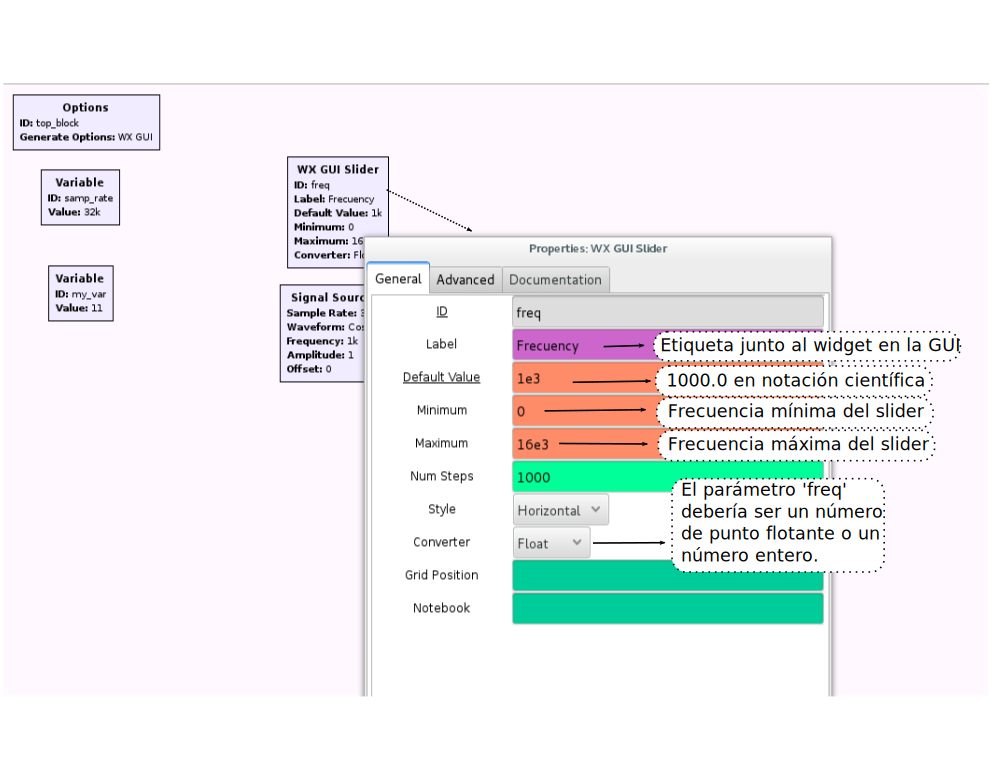
\includegraphics[width=\textwidth]{parte1/lab1/pdf/lab1_13.pdf}
\end{figure}
\end{frame}
%-----------------------------------

\begin{frame}{Primeros pasos }
\begin{figure}[H]
\vspace{-1cm}
\centering
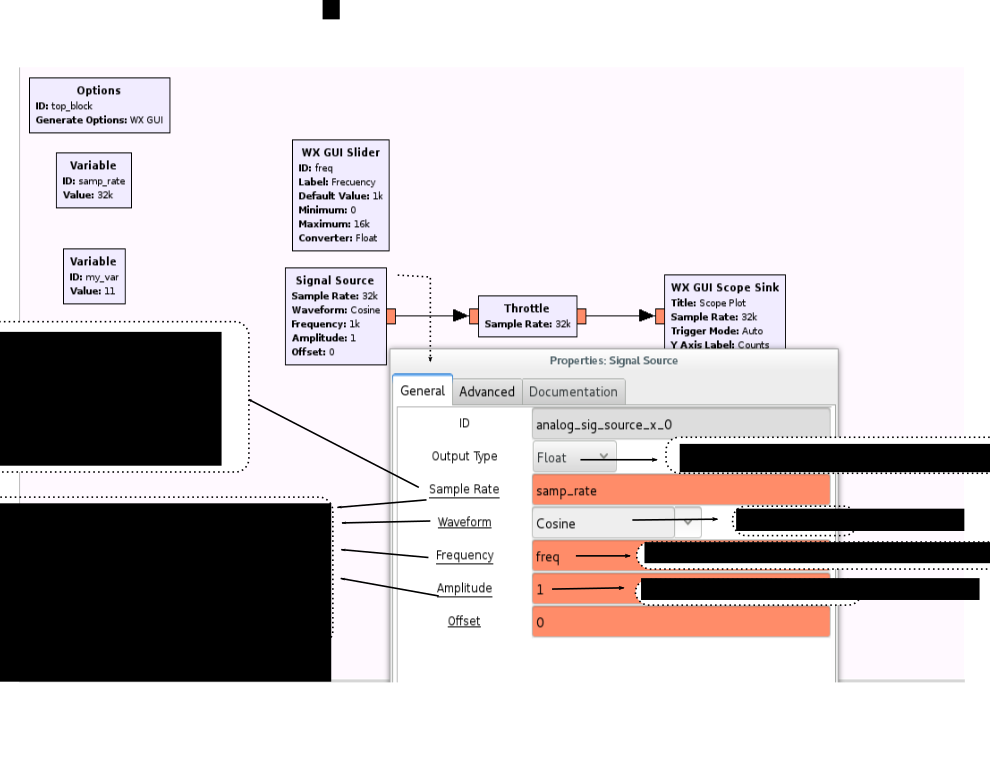
\includegraphics[width=1.05\textwidth]{parte1/lab1/pdf/lab1_14.pdf}
\end{figure}
\end{frame}
%-----------------------------------

\begin{frame}{Primeros pasos }
\begin{figure}[H]
\vspace{-3mm}
\centering
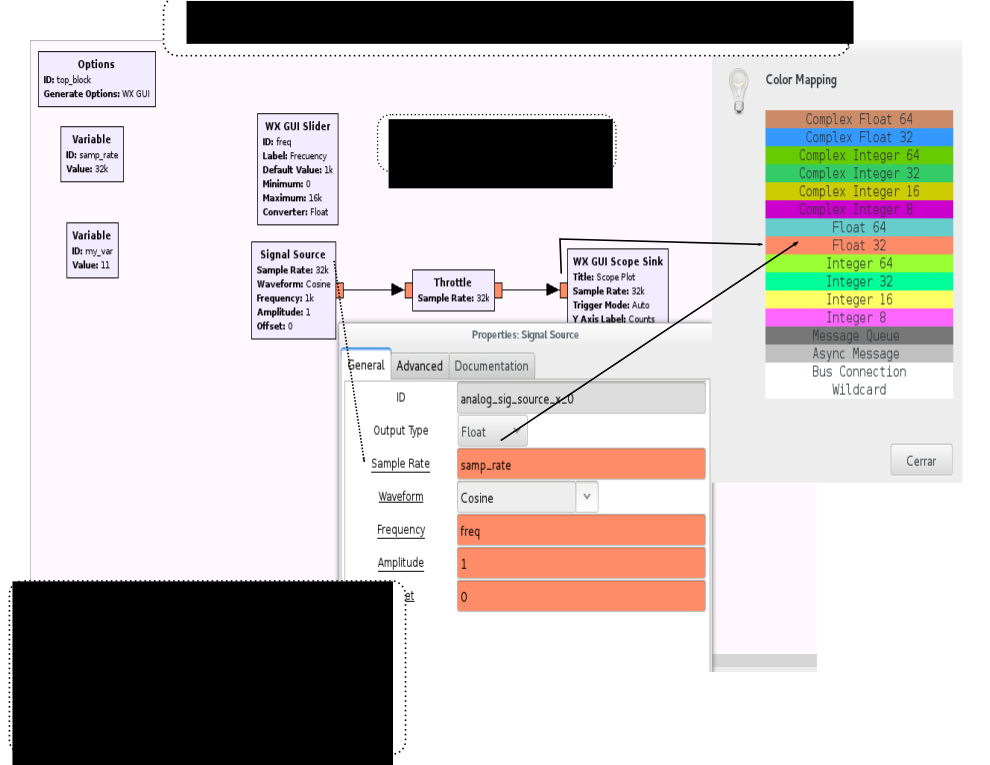
\includegraphics[width=.80\textwidth]{parte1/lab1/pdf/lab1_15.pdf}
\end{figure}
\end{frame}
%-----------------------------------

\begin{frame}{Primeros pasos }
\begin{figure}[H]
\centering
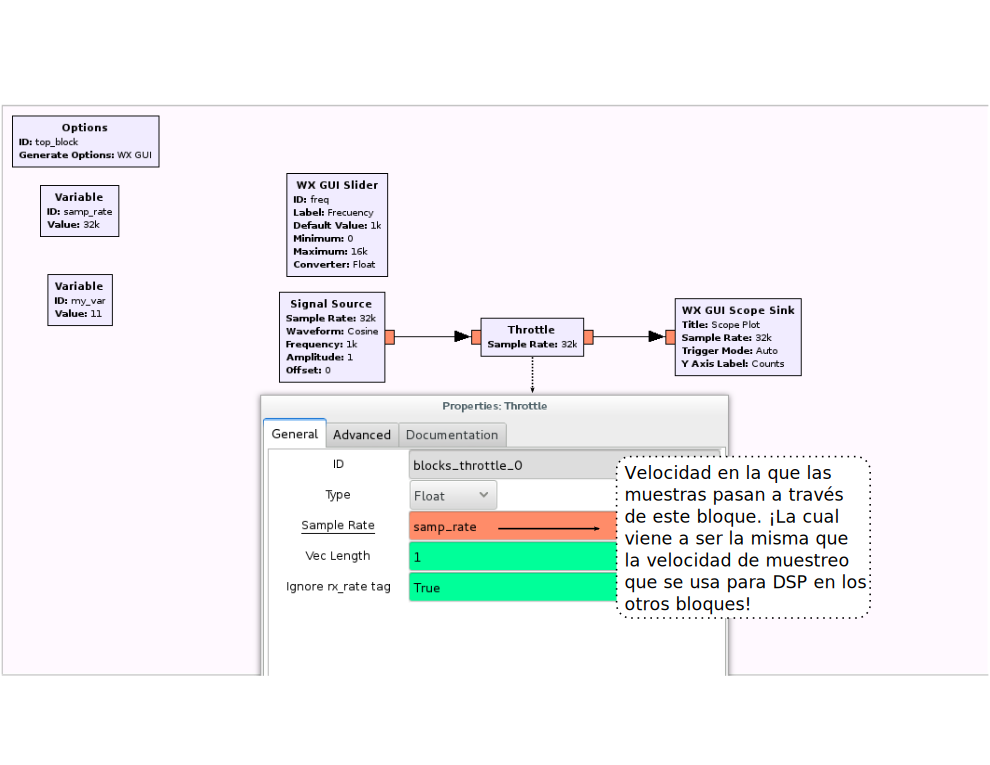
\includegraphics[width=\textwidth]{parte1/lab1/pdf/lab1_16.pdf}
\end{figure}
\end{frame}
%-----------------------------------

\begin{frame}{Primeros pasos }
\begin{figure}[H]
\vspace{-3mm}
\centering
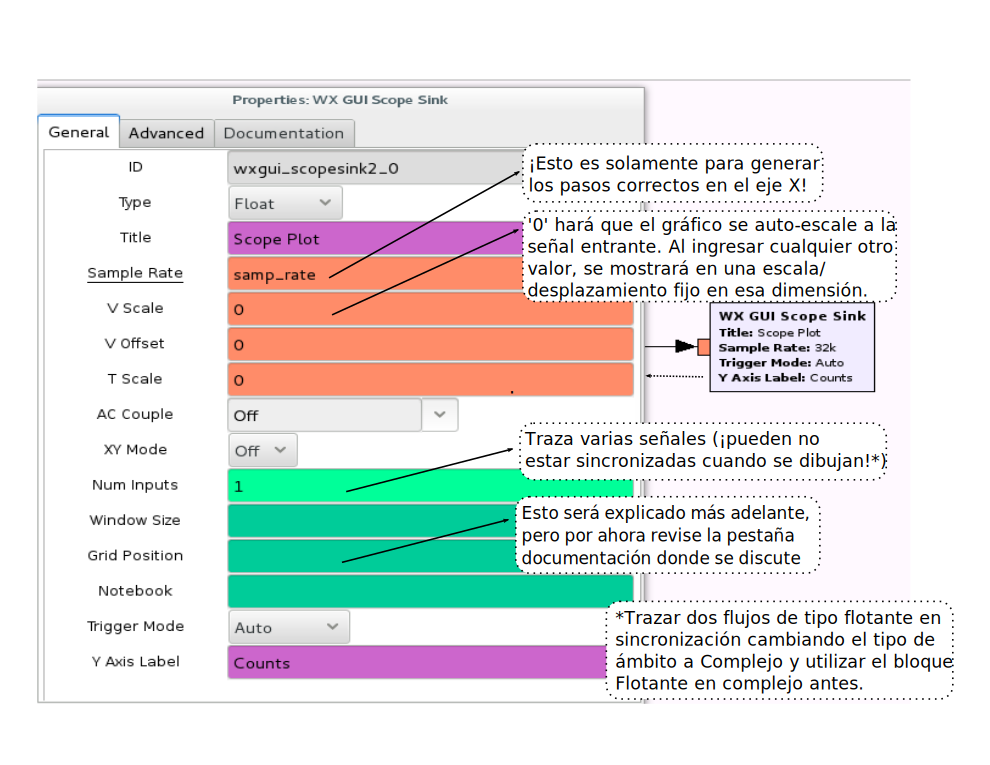
\includegraphics[width=.85\textwidth]{parte1/lab1/pdf/lab1_17.pdf}
\end{figure}
\end{frame}
%-----------------------------------

\begin{frame}{Primeros pasos }
\begin{figure}[H]
\centering
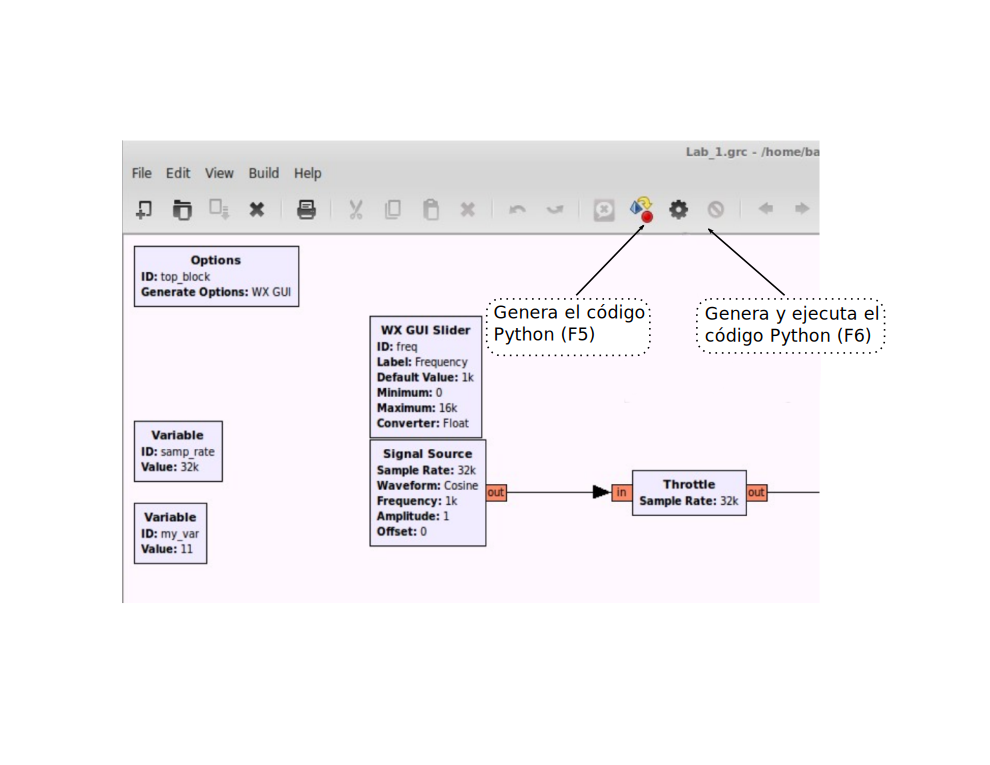
\includegraphics[width=\textwidth]{parte1/lab1/pdf/lab1_18.pdf}
\end{figure}
\end{frame}
%-----------------------------------

\begin{frame}{Primeros pasos }
Programa en Python generado por GRC
\begin{figure}[H]
\centering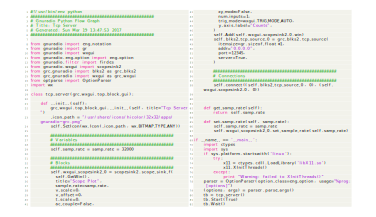
\includegraphics[width=0.95\textwidth]{parte1/lab1/pdf/lab1_18a.pdf}
\end{figure}
\end{frame}
%-----------------------------------

\begin{frame}{Primeros pasos }
\begin{figure}[H]
\centering
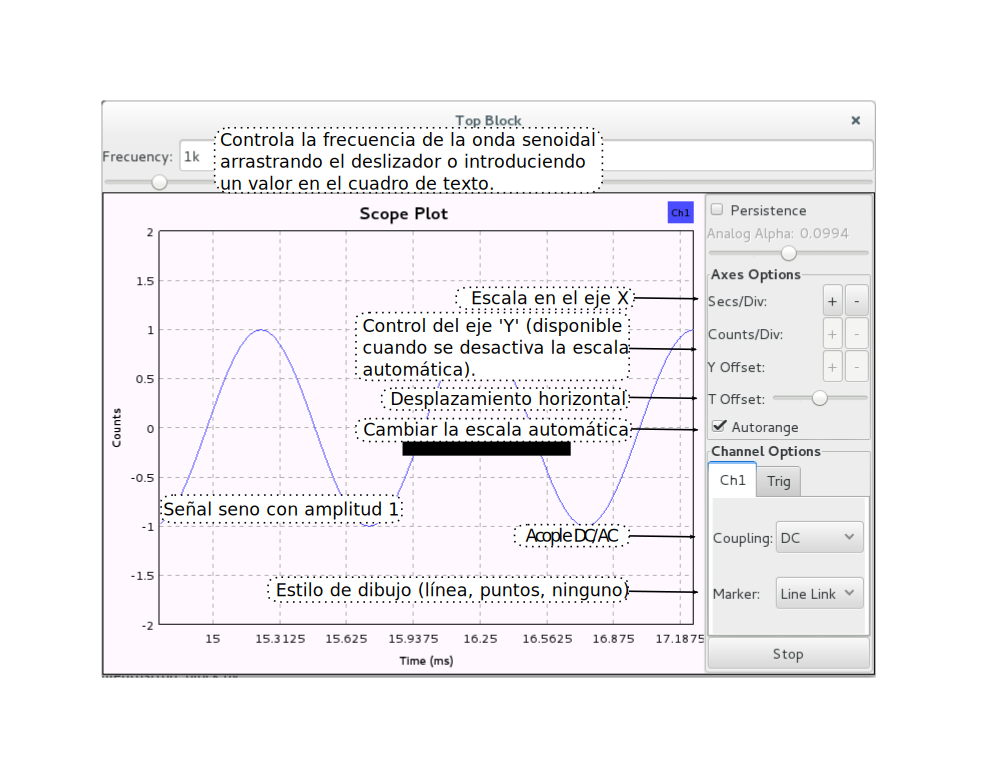
\includegraphics[width=\textwidth, height=0.55\textwidth]{parte1/lab1/pdf/lab1_19.pdf}
\end{figure}
\end{frame}
%-----------------------------------

\begin{frame}{Primeros pasos }
\begin{figure}[H]
\centering
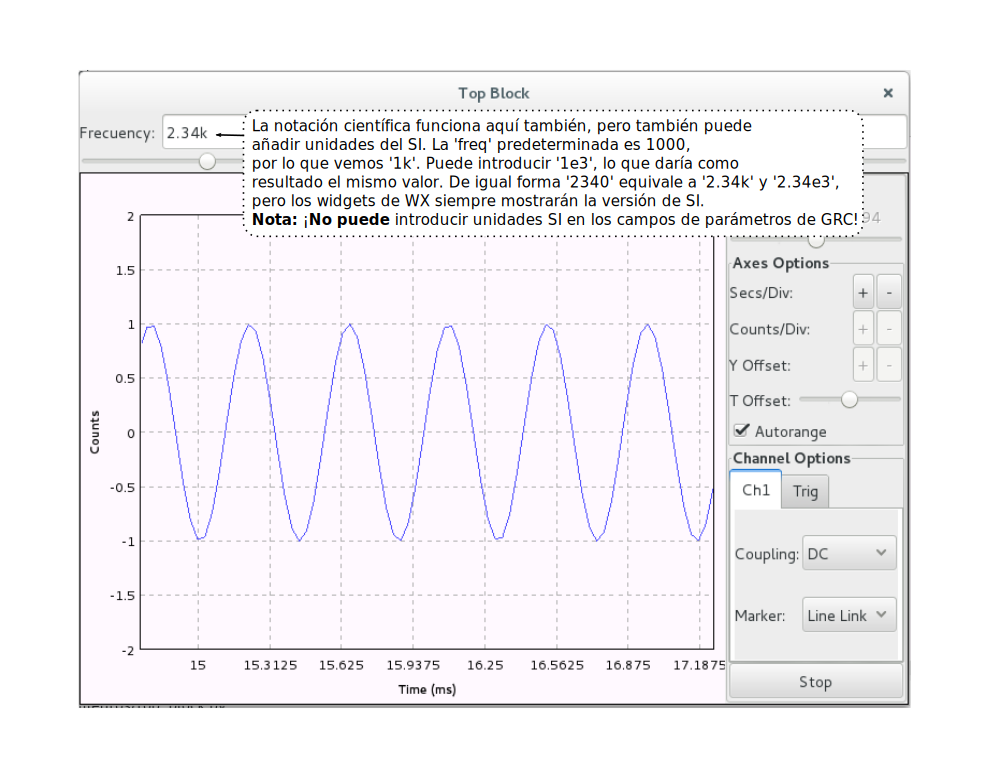
\includegraphics[width=\textwidth, height=0.55\textwidth]{parte1/lab1/pdf/lab1_20.pdf}
\end{figure}
\end{frame}
%-----------------------------------

\begin{frame}{Primeros pasos }
\begin{figure}[H]
\centering
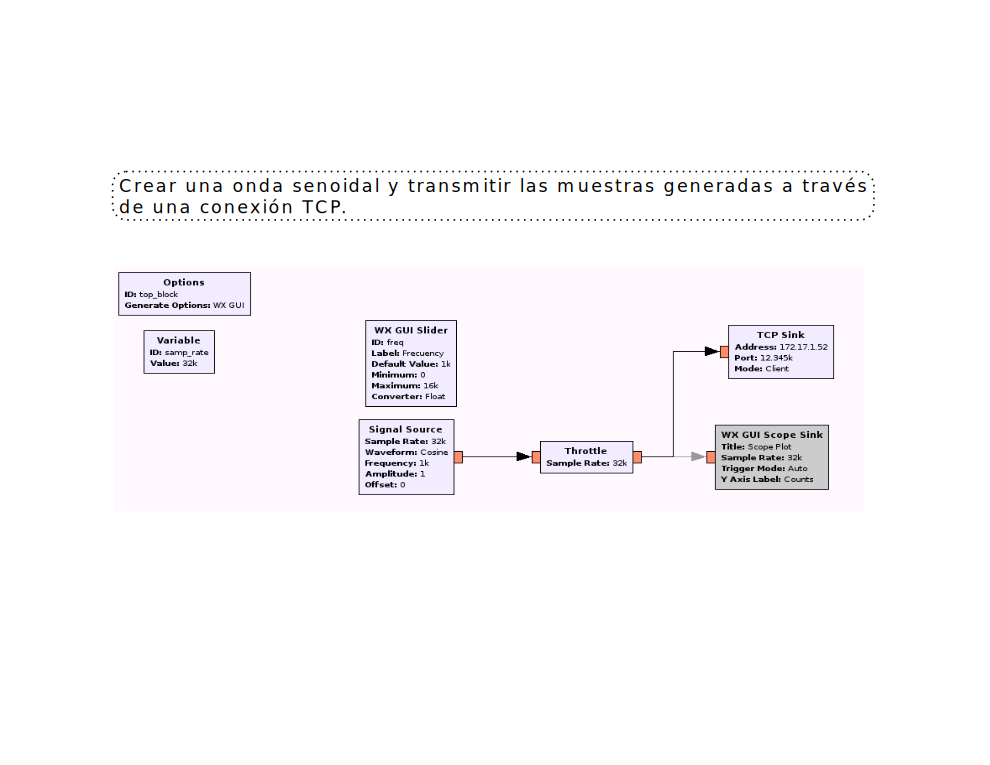
\includegraphics[width=\textwidth]{parte1/lab1/pdf/lab1_21.pdf}
\end{figure}
\end{frame}
%-----------------------------------

\begin{frame}{Primeros pasos }
\begin{figure}[H]
\centering
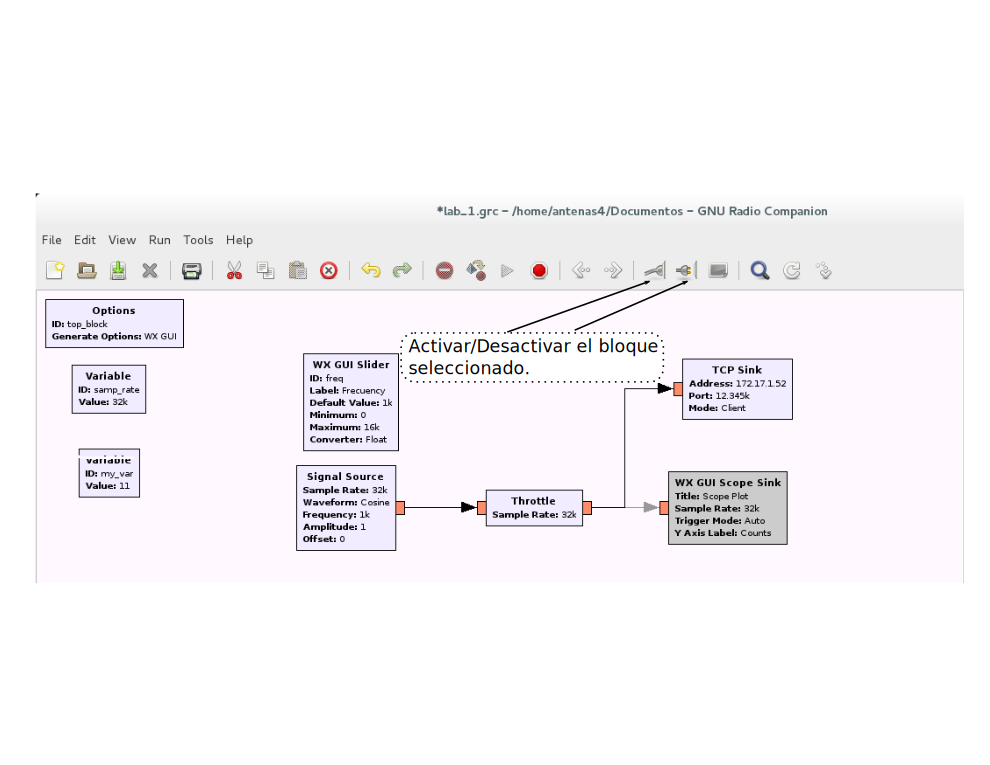
\includegraphics[width=\textwidth]{parte1/lab1/pdf/lab1_22.pdf}
\end{figure}
\end{frame}
%-----------------------------------

\begin{frame}{Primeros pasos }
\begin{figure}[H]
\centering
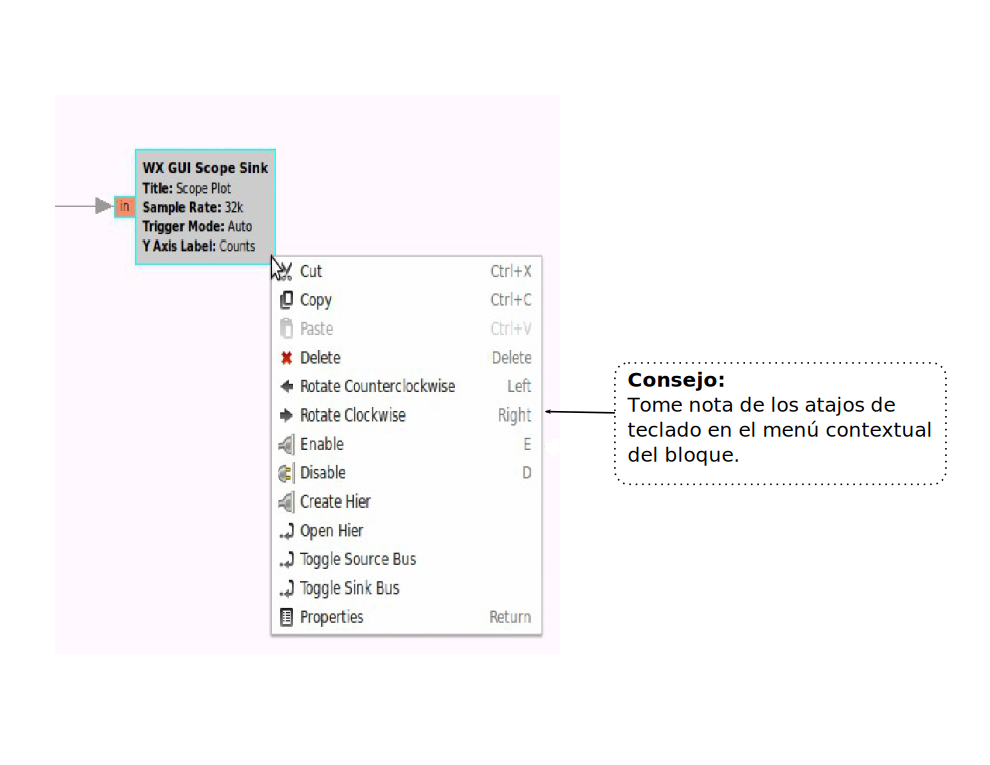
\includegraphics[width=\textwidth, height=0.6\textwidth]{parte1/lab1/pdf/lab1_23.pdf}
\end{figure}
\end{frame}
%-----------------------------------

\begin{frame}{Primeros pasos }
\begin{figure}[H]
\centering
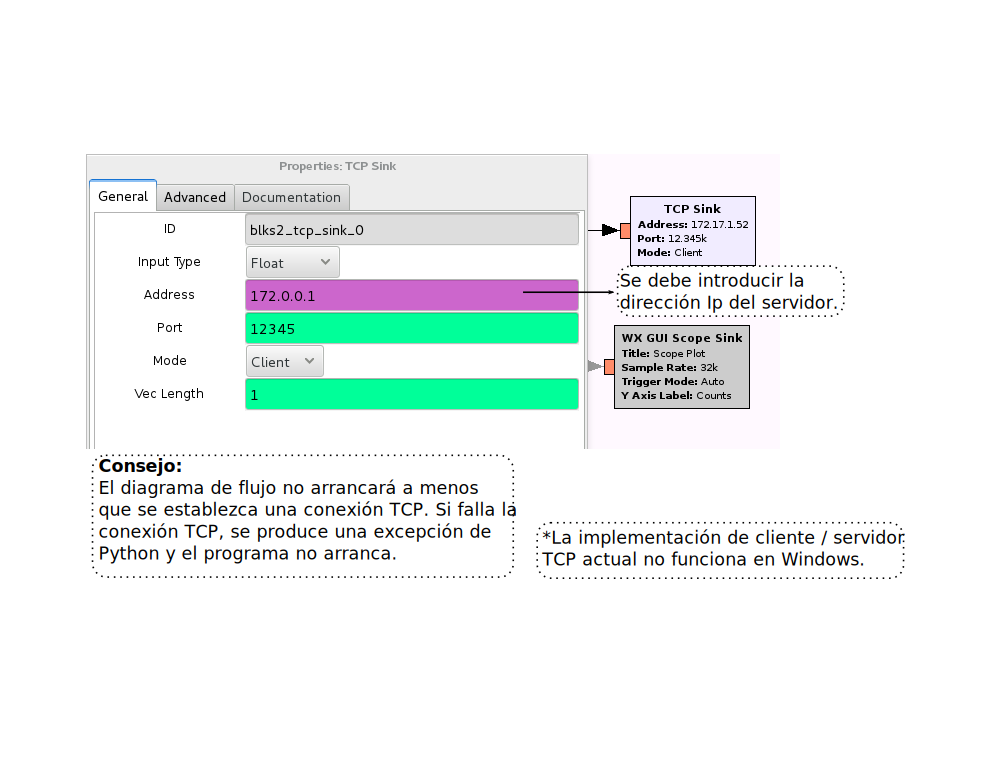
\includegraphics[width=\textwidth]{parte1/lab1/pdf/lab1_24.pdf}
\end{figure}
\end{frame}
%-----------------------------------

\begin{frame}{Primeros pasos }
\begin{figure}[H]
\centering
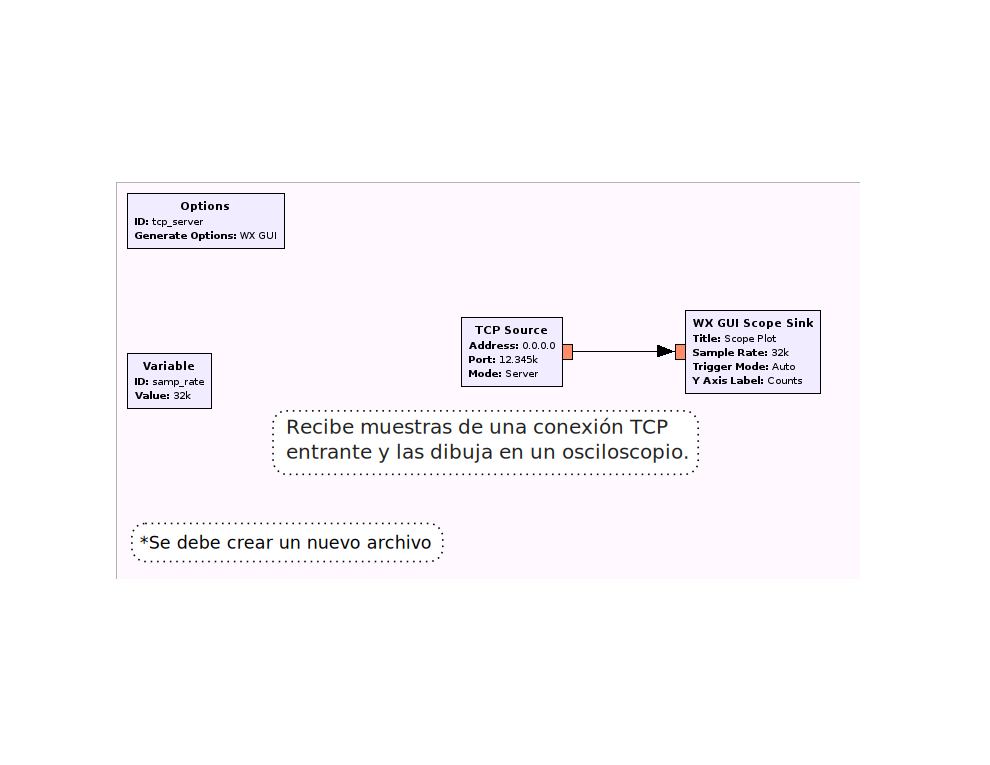
\includegraphics[width=\textwidth]{parte1/lab1/pdf/lab1_25.pdf}
\end{figure}
\end{frame}
%-----------------------------------

\begin{frame}{Primeros pasos }
\begin{figure}[H]
\centering
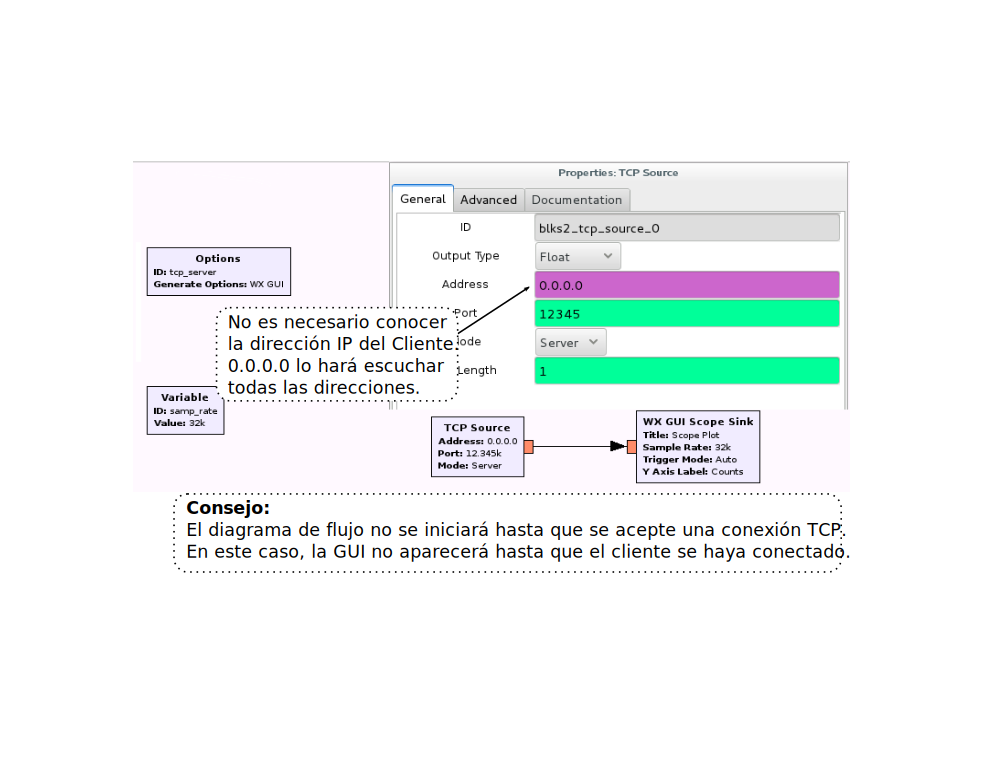
\includegraphics[width=\textwidth]{parte1/lab1/pdf/lab1_26.pdf}
\end{figure}
\end{frame}
%-----------------------------------

\begin{frame}{Primeros pasos }
\begin{figure}[H]
\centering
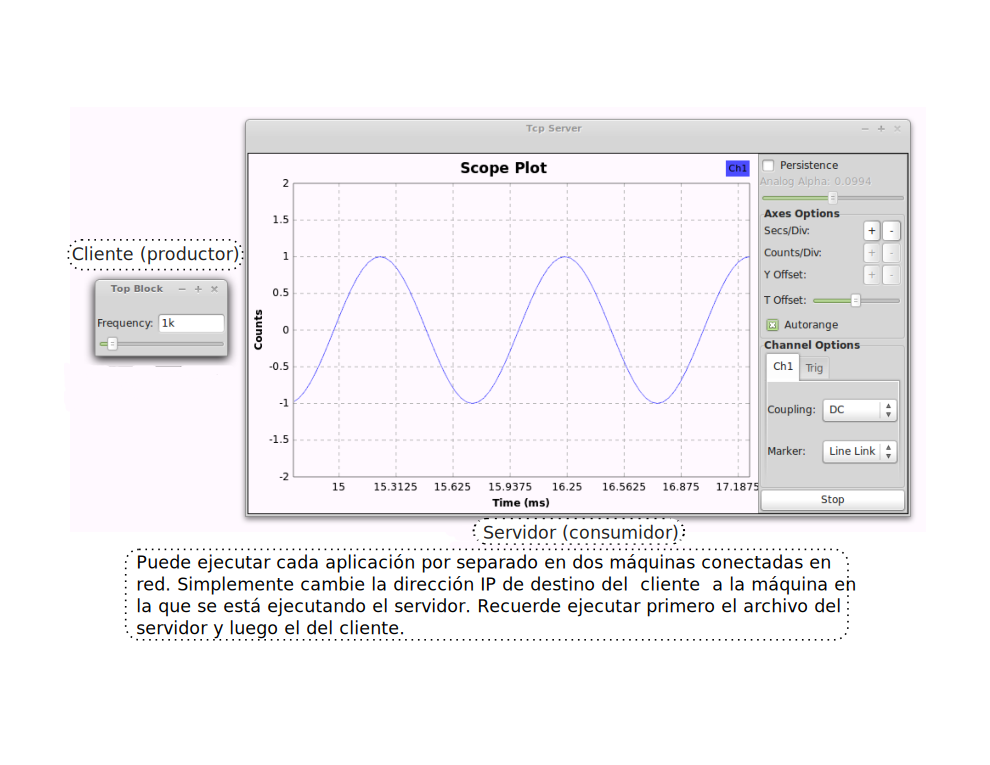
\includegraphics[width=\textwidth, height=0.55\textwidth]{parte1/lab1/pdf/lab1_27.pdf}
\end{figure}
\end{frame}
%-----------------------------------

\subsubsection{Actividad 1_lab1}
\begin{frame}

\pgfdeclareimage[width=\paperwidth,height=\paperheight]{bg}{imagenes/fondo_seccion}
\setbeamertemplate{background}{\pgfuseimage{bg}}

\definecolor{greenU}{RGB}{212,202,72}
\setbeamercolor{block body}{fg=Black,bg=greenU}
\begin{block}{}
	\centering
	%\vspace{1mm}
	\Large{\textit{Actividades}}
	%\vspace{1mm}
\end{block}
\end{frame}

\begin{frame}

\pgfdeclareimage[width=\paperwidth,height=\paperheight]{bg}{imagenes/fondo3}
\setbeamertemplate{background}{\pgfuseimage{bg}}

\frametitle{\underline{\textbf{Transmisión de señales por multiplexación}}}

En esta actividad usted debe transmitir 3 señales periódicas por medio del TCP (Protocolo de 	Control de Transmisión) desde el cliente, mediante el proceso de multiplexación de señales, al 	servidor, que se encargará de demultiplexar la señal recibida y mostrar las 3 que fueron  	transmitidas en el Scope Sink.\vspace{2mm}

Es importante saber que:
\begin{enumerate}[1.]
\item {La multiplexación es el proceso mediante el cual diferentes mensajes de información (Señales) se combinan en una única señal con el fin de trasmitirla. }\\

\item {La demultiplexación es el proceso mediante el cual la señal multiplexada recibida se divide en cada una de las señales que la generaron.}\\
\end{enumerate}
\end{frame}

%-----------------------------------

\begin{frame}

\pgfdeclareimage[width=\paperwidth,height=\paperheight]{bg}{imagenes/fondo3}
\setbeamertemplate{background}{\pgfuseimage{bg}}

\frametitle{\underline{\textbf{Pistas para la actividad}}}

Las pistas son:
\begin{enumerate}[1.]
	\item {Modo cliente: Bloques y conexiones de los primeros pasos. (WX GUI Slider, Signal Source, TCP Sink, Scope Sink, Throttle, Stream Mux, Variable)}
	
	\item {Modo servidor:  Bloques y conexiones de los primeros pasos. (TCP Source, Scope Sink, Stream to Streams)}
	\item {Multiplexación: Bloque Stream Mux. En el parámetro Lengths se debe agregar el número de ítems de cada señal, en forma de lista. Para la actividad las señales cuentan con un solo ítem. 
	Como ejemplo de lo anterior tenemos que: }
\begin{itemize}
	\item 2 señales = 1,1    
	\item 3 señales = 1,1,1 
	\item 4 señales = 1,1,1,1
\end{itemize}
	\item {Demultiplexación: Bloque Stream to Streams.}
    \item { El tipo de dato en todos los bloques debe ser el mismo. (float)}
	\item {Habilitar las entradas o salidas suficientes para los bloques.}
\end{enumerate}
\end{frame}

%-----------------------------------

%\begin{frame}{Actividad de los Primeros pasos }
%\begin{figure}[H]
%\centering
%\vspace{-3mm}
%\includegraphics[width=0.9\textwidth]{parte1/lab1/Actividades/pdf/prueba.pdf}
%\end{figure}
%\end{frame}
%-----------------------------------

\subsubsection{Actividad2}


\begin{frame}
	\frametitle{\underline{\textbf{Modificación de las variables de una señal periódica}}}
	
	Aprender a variar los componentes básicos de una señal periódica (amplitud, frecuencia, fase y nivel DC) en GNU Radio.\vspace{2mm}
	
	Es importante saber que:
	
	\begin{enumerate}[1.]
		\item{La forma más simple de representar una señal periódica es una senoidal como se presenta matemáticamente a continuación}\\
		
		$$x(t)=A\sin(2 \pi f + \phi) + K$$\\
		
		En donde:\\
		
		\item{Amplitud ($A$): Es el valor máximo que toma la señal, es decir, la distancia entre el punto máximo de la señal y cero, este punto puede ser tanto positivo como negativo.}\\
		
		\item{Frecuencia ($f$): Es el número de ciclos que realiza la señal por unidad de tiempo, esta medida está dada en Hertz (Hz), que equivale a un ciclo por segundo, lo que significa que 80 Hz son 80 ciclos por cada segundo que transcurre.}\\
		
	\end{enumerate}
\end{frame}


\begin{frame}
	\frametitle{\underline{\textbf{Modificación de las variables de una señal periódica}}}
	\begin{enumerate}[1.]
		
		\item{La fase ($\phi$): Indica la magnitud de una de variación ciclíca, siendo la fracción del período que transcurre desde el instante tomado al estado hasta la referencia, es decir el desplazamiento que tiene una señal en grados con respecto a su referencia.}\\
		
		\item{Nivel DC ($K$): Es el valor medio de la señal, lo que quiere decir que es un voltaje en DC que se le suma a la señal AC, para obtener un desplazamiento en la amplitud de la señal, puede ser tanto positivo como negativo.}\\
		
	\end{enumerate}
\end{frame}

\begin{frame}{Actividad}
	\begin{enumerate}[1.]
		
		\item{Realizar un programa que permita variar los componentes básicos de una señal periódica (amplitud, frecuencia, fase y nivel DC) en GNU Radio.}\\
		
	\end{enumerate}
\end{frame}

\begin{frame}
	
	\frametitle{\underline{\textbf{Pistas para la actividad}}}
	
	Las pistas son:
	\begin{enumerate}[1.]
		
		\item {Repasar los bloques utilizados en la primera guía "Primeros pasos"}\\
		\item {Debe existir un WX GUI Slider para cada variable que se desee modificar en el osciloscopio.}\\
		\item {Para una mejor apreciación  de los cambios en las variables de la señal se sugiere añadir otra señal que sirva como referencia}\\
		\item {Coherencia entre los tipos de dato entre bloques}\\
		\item {Para variar el nivel DC de la señal, el oscilocopio debe tener la opción "Coupling" en DC}\\
		
	\end{enumerate}
\end{frame}



%///////////////////////////////////////////////////////////////

\subsection{Lab2: Osciloscopio y FFT}
%*********************
\begin{frame}{}

\pgfdeclareimage[width=\paperwidth,height=\paperheight]{bg}{imagenes/fondo_lab}
\setbeamertemplate{background}{\pgfuseimage{bg}}

\bfseries{\textrm{\LARGE Lab2\\ \Large Osciloscopio y FFT}}
\raggedright
\end{frame}
%*********************

%-----------------------------------
\begin{frame}{Osciloscopio y FFT\index{TCP}}

\pgfdeclareimage[width=\paperwidth,height=\paperheight]{bg}{imagenes/fondo3}
\setbeamertemplate{background}{\pgfuseimage{bg}}

En este laboratorio se genera una onda senoidal y a su vez algún ruido; estas dos señales se suman y se observa el resultado en el dominio de la frecuencia (FFT) y del tiempo (Scope). Se aprende a utilizar el notebook y algunas herramientas básicas del GRC. 

\end{frame}
%---------------------------------

\begin{frame}{Osciloscopio y FFT\index{TCP}}

\begin{figure}[H]
\vspace{-4mm}
\centering
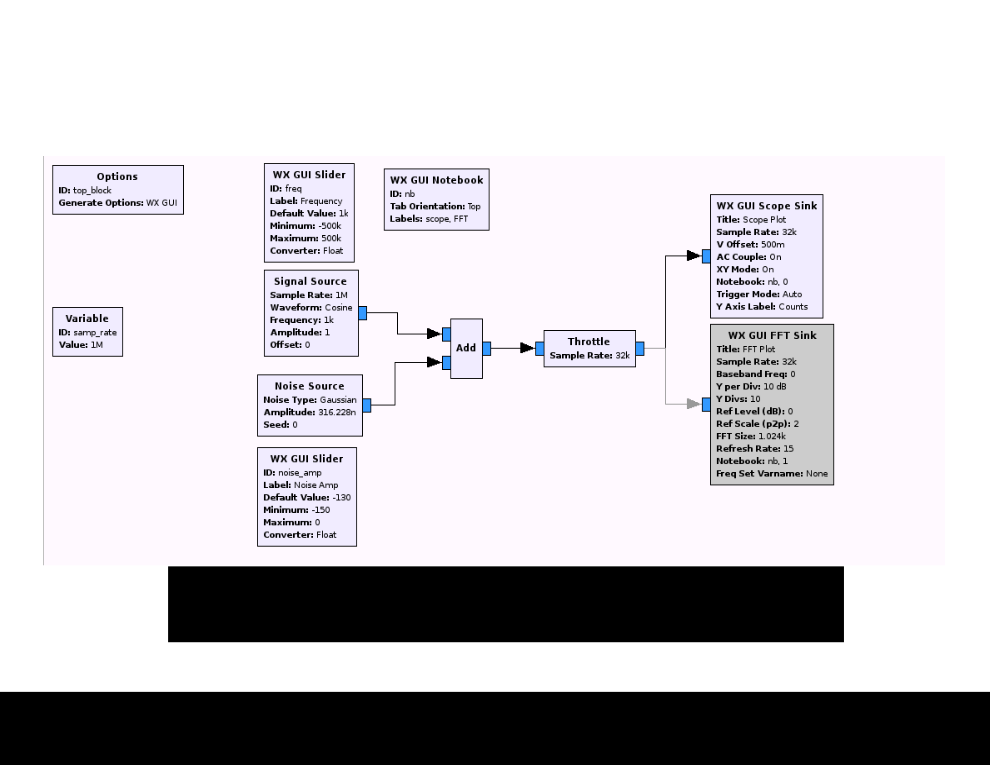
\includegraphics[width=1.2\textwidth]{parte1/lab2/pdf/lab2_1.pdf}
\end{figure}
\end{frame}
%---------------------------------

\begin{frame}{Osciloscopio y FFT}
\begin{figure}[H]
\vspace{-4mm}
\centering
\includegraphics[width=1.1\textwidth]{parte1/lab2/pdf/lab2_2.pdf}
\end{figure}
\end{frame}
%--------------------------------

\begin{frame}{Osciloscopio y FFT\index{Noise Source}}
\begin{figure}[H]
\centering
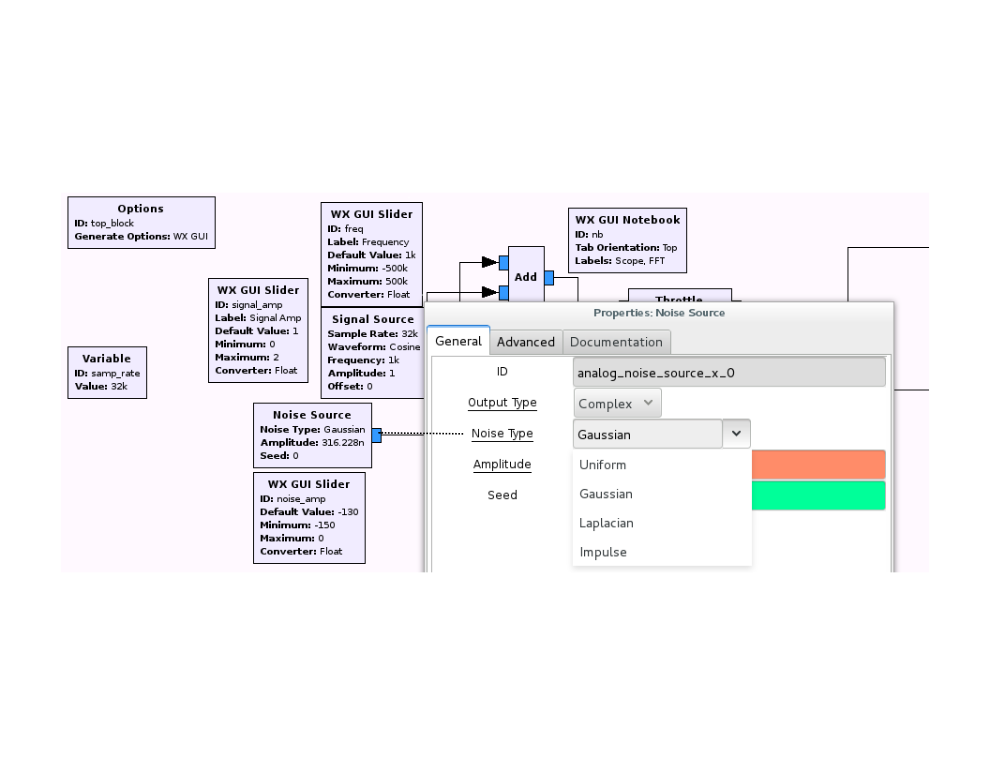
\includegraphics[width=1.055\textwidth]{parte1/lab2/pdf/lab2_3.pdf}
\end{figure}
\end{frame}
%--------------------------------

\begin{frame}{Osciloscopio y FFT\index{Noise Source}}
\begin{figure}[H]
\centering
\includegraphics[width=1.055\textwidth]{parte1/lab2/pdf/lab2_4.pdf}
\end{figure}
\end{frame}
%--------------------------------

\begin{frame}{Osciloscopio y FFT\index{Add}}
\begin{figure}[H]
\centering
\includegraphics[width=.7\textwidth]{parte1/lab2/pdf/lab2_5.pdf}
\end{figure}
\end{frame}
%--------------------------------

\begin{frame}{Osciloscopio y FFT}
\begin{figure}[H]
\vspace{-4mm}
\centering
\includegraphics[width=1.1\textwidth]{parte1/lab2/pdf/lab2_6.pdf}
\end{figure}
\end{frame}
%--------------------------------

\begin{frame}{Osciloscopio y FFT\index{WX GUI Notebook}}
\begin{figure}[H]
\vspace{-4mm}
\centering
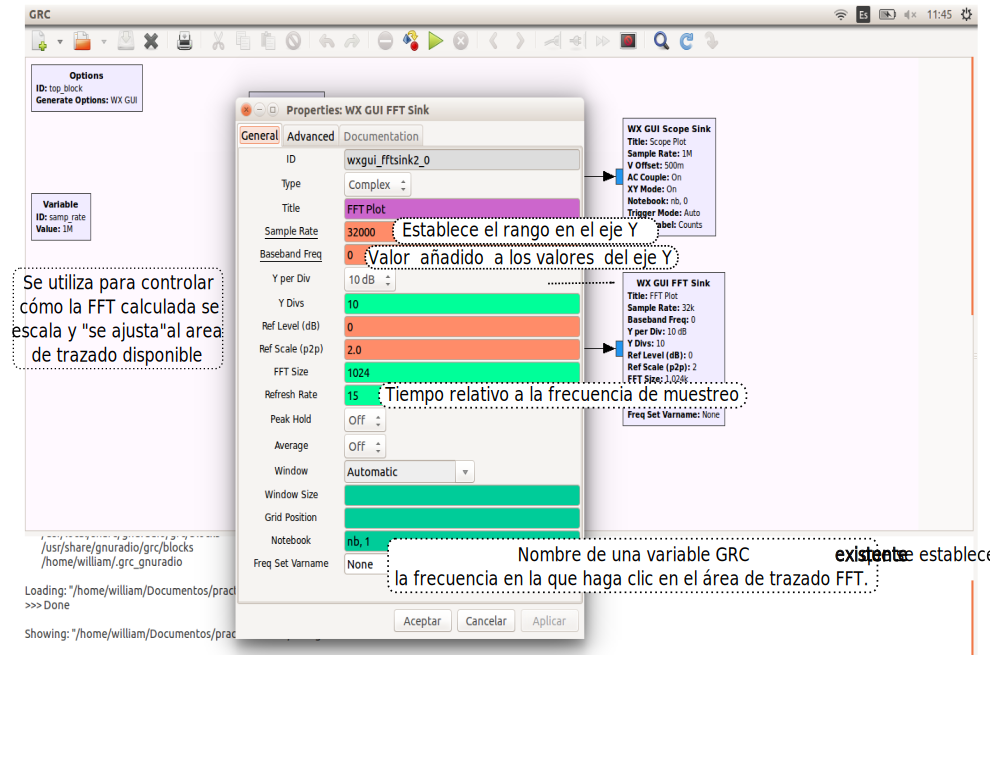
\includegraphics[width=0.85\textwidth]{parte1/lab2/pdf/lab2_7.pdf}
\end{figure}
\end{frame}
%--------------------------------

\begin{frame}{Osciloscopio y FFT\index{WX GUI FFT Sink}}
\begin{figure}[H]
\centering
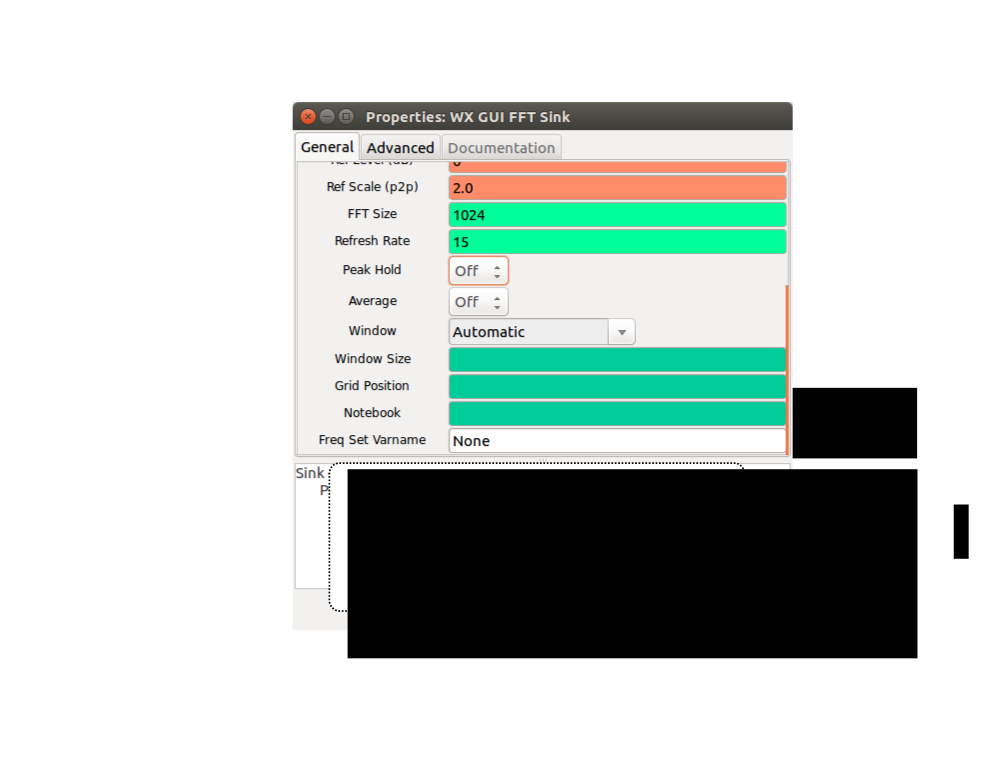
\includegraphics[width=1.1\textwidth]{parte1/lab2/pdf/lab2_8.pdf}
\end{figure}
\end{frame}
%--------------------------------

\begin{frame}{Osciloscopio y FFT\index{WX GUI FFT Sink}}
\begin{figure}[H]
\vspace{-3mm}
\centering
\includegraphics[width=0.7\textwidth]{parte1/lab2/pdf/lab2_9.pdf}
\end{figure}
\end{frame}
%--------------------------------

\begin{frame}{Osciloscopio y FFT}
\begin{figure}[H]
\vspace{-3mm}
\centering
\includegraphics[width=0.85\textwidth]{parte1/lab2/pdf/lab2_10.pdf}
\end{figure}
\end{frame}
%--------------------------------

\begin{frame}{Osciloscopio y FFT}
\begin{figure}[H]
\vspace{-3mm}
\centering
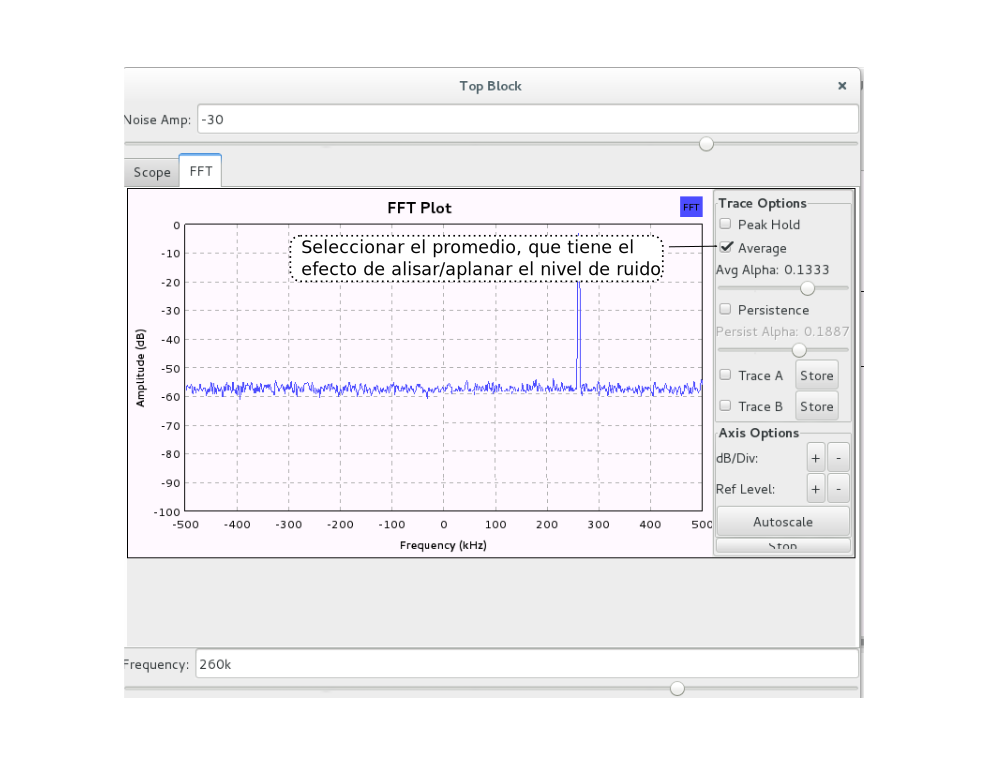
\includegraphics[width=0.75\textwidth]{parte1/lab2/pdf/lab2_11.pdf}
\end{figure}
\end{frame}
%--------------------------------

\begin{frame}{Osciloscopio y FFT}
\begin{figure}[H]
\vspace{-3mm}
\centering
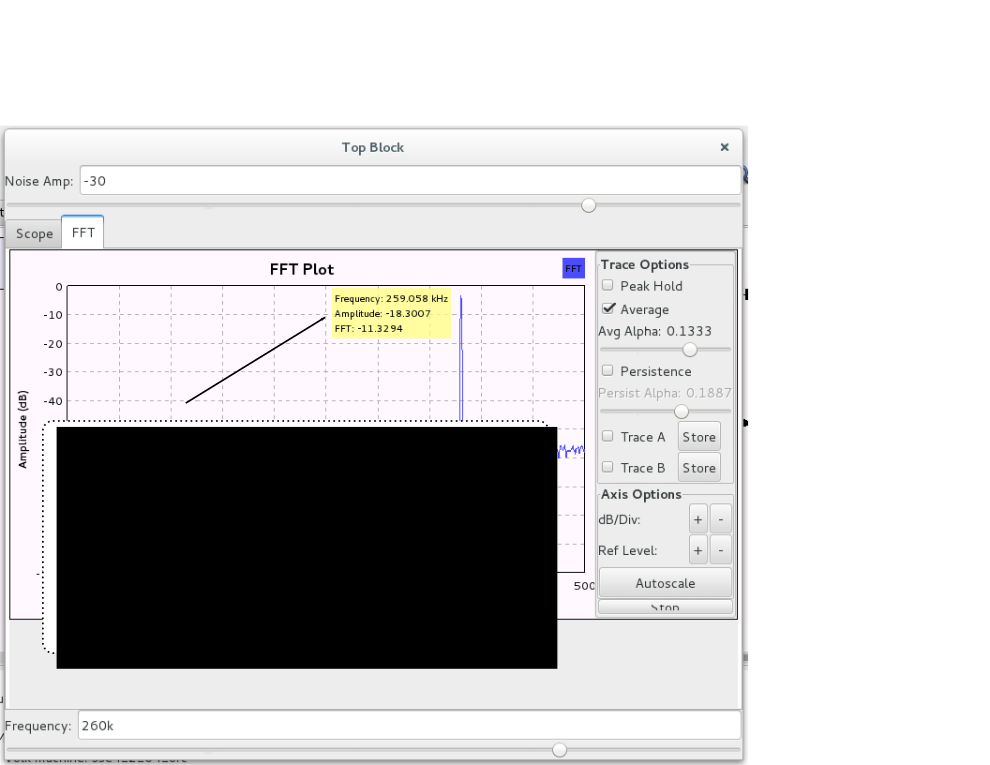
\includegraphics[width=0.75\textwidth]{parte1/lab2/pdf/lab2_12.pdf}
\end{figure}
\end{frame}
%--------------------------------

\begin{frame}{Osciloscopio y FFT}
\begin{figure}[H]
\centering
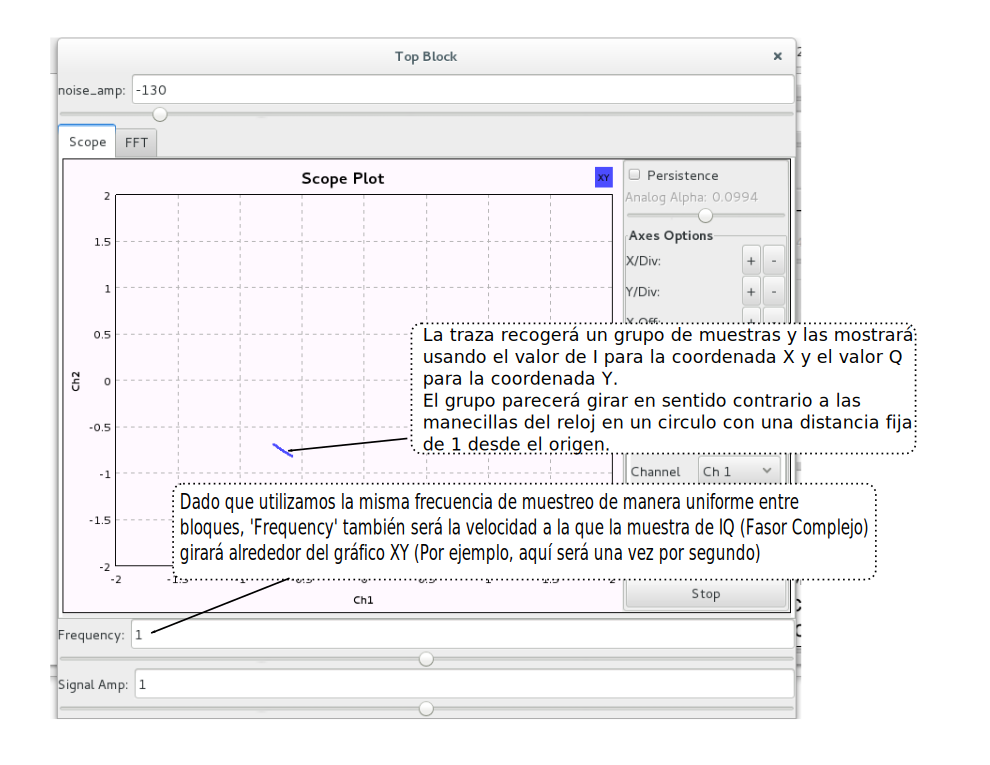
\includegraphics[width=0.75\textwidth]{parte1/lab2/pdf/lab2_13.pdf}
\end{figure}
\end{frame}
%--------------------------------

\begin{frame}{Osciloscopio y FFT}
\begin{figure}[H]
\vspace{-3mm}
\centering
\includegraphics[width=0.75\textwidth]{parte1/lab2/pdf/lab2_14.pdf}
\end{figure}
\end{frame}
%--------------------------------

\begin{frame}{Osciloscopio y FFT}
\begin{figure}[H]
\vspace{-3mm}
\centering
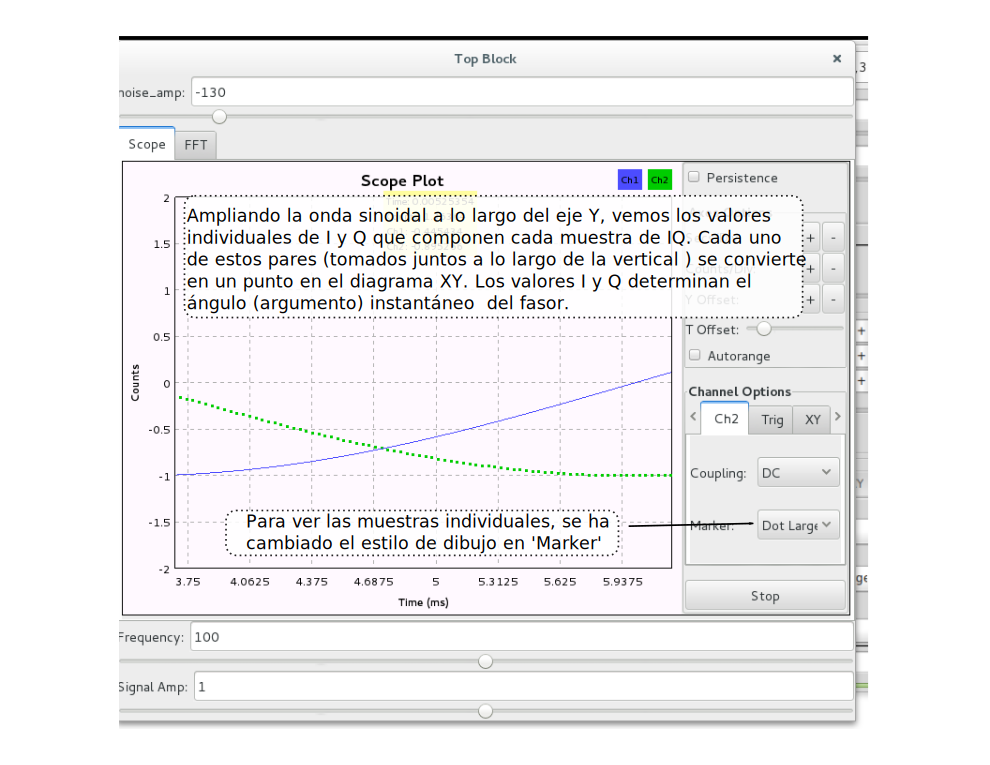
\includegraphics[width=0.7\textwidth]{parte1/lab2/pdf/lab2_15.pdf}
\end{figure}
\end{frame}
%--------------------------------

\begin{frame}{Osciloscopio y FFT}
\begin{figure}[H]
\centering
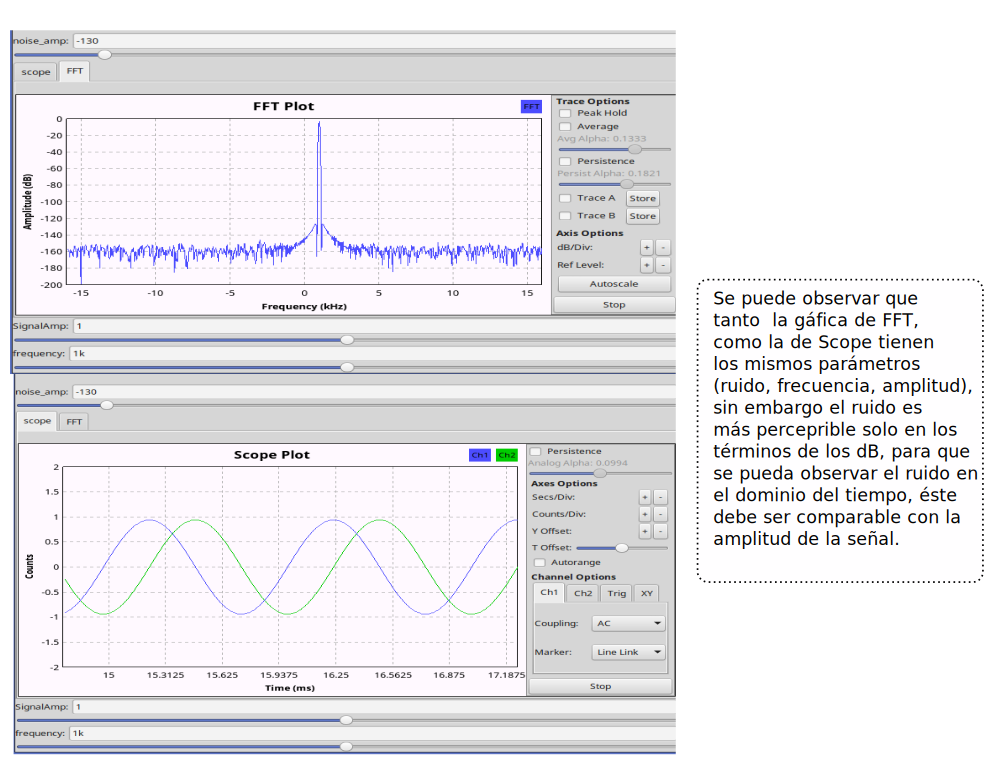
\includegraphics[width=\textwidth, height=0.58\textwidth]{parte1/lab2/pdf/lab2_16.pdf}
\end{figure}
\end{frame}
%--------------------------------

%\usepackage{amssymb}
%\usepackage{amsmath}
\subsubsection{Actividad 1 lab 2}
%*********************
\begin{frame}{}

\pgfdeclareimage[width=\paperwidth,height=\paperheight]{bg}{imagenes/fondo_seccion}
\setbeamertemplate{background}{\pgfuseimage{bg}}

\definecolor{greenU}{RGB}{212,202,72}
\setbeamercolor{block body}{fg=Black,bg=greenU}
\begin{block}{}
	\centering
	\vspace{1mm}
	\large{\textit{Actividades}}
	\vspace{1mm}
\end{block}
\end{frame}
%*********************


%--------------------------------
\begin{frame}{Actvidad 1 lab 2}
\begin{figure}[H]
\begin{flushleft}
Mencione los diferentes tipos de ruido del bloque (noise source), sus características,
describa la función de densidad de probabilidad para cada uno de estos y por que se puede ocasionar
\end{flushleft}
\centering
\includegraphics[width=\textwidth, height=0.58\textwidth]{parte1/lab2/pdf/lab2_17.pdf}
\end{figure}
\end{frame}
%--------------------------------


\subsubsection{Actividad 2 lab 2}
%*********************

\begin{frame}{Actvidad 2 lab 2}
\begin{figure}[H]
\begin{flushleft}
Objetivos:
\end{flushleft}
\begin{flushleft}
-Dar a conocer a lector la distribución  de los diferentes tipos de ruido y sus propiedades.
\end{flushleft}
\begin{flushleft}
-Relacionar las funciones de densidad con cada uno de los diferentes ruidos que aparecen en el modulo noise source.
\end{flushleft}
\begin{flushleft}
-Mediante una breve configuración al lab 2 compare y evidencie que lo anterior se cumpla.
\end{flushleft}

\begin{center}
\centering
\includegraphics[width=\textwidth, height=0.58\textwidth]{parte1/lab2/pdf/lab2_18.pdf}
\end{center}
\end{figure}
\end{frame}
%--------------------------------

\subsubsection{Actividad 2 lab 3}
%*********************
%--------------------------------
\begin{frame}{Actvidad 3 lab 2}
\begin{figure}[H]
\begin{flushleft}
Objetivo:
\end{flushleft}
\begin{flushleft}
-Variar la  amplitud y fase de la señal para generar las curvas de Lissajous.
\end{flushleft}

\begin{center}
\centering
\includegraphics[width=0.65\textwidth]{parte1/lab2/pdf/lab2_19.pdf}
\end{center}
\end{figure}
\end{frame}
%--------------------------------


%///////////////////////////////////////////////////////////////

\subsection{Lab3: Audio}
%*********************
\begin{frame}{}

\pgfdeclareimage[width=\paperwidth,height=\paperheight]{bg}{imagenes/fondo_lab}
\setbeamertemplate{background}{\pgfuseimage{bg}}

\bfseries{\textrm{\LARGE Lab3\\ \Large Audio}}
\raggedright
\end{frame}
%*********************

\begin{frame}{Audio \index{Audio}}

\pgfdeclareimage[width=\paperwidth,height=\paperheight]{bg}{imagenes/fondo3}
\setbeamertemplate{background}{\pgfuseimage{bg}}


En esta práctica se generará un tono desde la tarjeta de sonido de la computadora, originado desde el software y emitido a través de los parlantes del computador, dicha señal será visualizada desde un osciloscopio, un FFT, y diagrama de cascada (espectrograma), realizando pruebas de "loopback" usando el micrófono de la computadora.

\end{frame}
%----------------

\begin{frame}{Diagrama:  “emisión de audio desde la computadora”\index{Audio}}

\begin{figure}

\begin{center}
\vspace{-0.3cm}
\includegraphics[width=.7\textwidth]{parte1/lab3/pdf/lab3_1.pdf}
\end{center}
\end{figure}

\end{frame}
%----------------

\begin{frame}{Diagrama:  “emisión de audio desde la computadora”\index{Audio}}

\begin{figure}

\begin{center}
\vspace{-2mm}
    \includegraphics[width=.85\textwidth]{parte1/lab3/pdf/lab3_2.pdf}
\end{center}
\end{figure}

\end{frame}
%----------------

\begin{frame}{Diagrama:  “emisión de audio desde la computadora”\index{Audio}}

\begin{figure}

\begin{center}
\vspace{-1mm}
\includegraphics[width=.92\textwidth]{parte1/lab3/pdf/lab3_3.pdf}
\end{center}
\end{figure}

\end{frame}
%----------------

\begin{frame}{Diagrama:  “emisión de audio desde la computadora”\index{Audio}}

\begin{figure}

\begin{center}
\vspace{-8mm}
\includegraphics[width=1.05\textwidth]{parte1/lab3/pdf/lab3_4.pdf}
\end{center}
\end{figure}

\end{frame}
%----------------

\begin{frame}{Audio\index{Audio}}

Es importante saber que:\\
\begin{itemize}
    \item
    {Cuando Audio Sink es el único dispositivo hardware en el diagrama de bloques capaz de generar audio, el modo de bloqueo (‘OK to Block’) aplicará un regulador a la producción de muestras del sample\_rate, para que opere eficazmente al reproducir el sonido\cite{Seeber2014}.}
    \item
    {Esto puede ser problemático si la fuente del diagrama de flujo es, por ejemplo, un RTL-SDR. La fuente es también un hardware que tiene su propio reloj interno y será regulado a la tasa de producción de las muestras, mientras que el Audio Sink regula el uso con su propio reloj no sincronizado. Esto se llama el problema de “dos relojes".}
\end{itemize}
\end{frame}
%----------------

\begin{frame}{Audio\index{Audio}}
\begin{itemize}
    \item 
    {Para solucionar este problema de dos relojes, se coloca un regulador de audio en modo sin bloqueo (no dar click ‘Botón de Bloqueo’) de tal forma que nunca interrumpa el diagrama de bloque (es decir, no aplicar el regulador controlado). Esto usará muestras de forma normal, pero si hay un exceso (por ejemplo, el RTL-SDR está produciendo muestras un poco más rápido de lo que el Audio Sink puede usar), se perderán las muestras (podría causar fallas de audio).}
    \item 
    {Esto no soluciona el caso en el que las muestras se producen más lentamente que la tasa de uso del Audio Sink (esto producirá una ejecución lenta: el audio sonará agitado y se imprimirá ‘aU’ en la ventana de registro).}
\end{itemize}



\end{frame}
%----------------

\begin{frame}{Audio\index{Audio}}

\begin{figure}

\begin{center}
\vspace{-7mm}
\includegraphics[width=\textwidth, height=0.6\paperheight]{parte1/lab3/pdf/lab3_5.pdf}
\end{center}
\end{figure}
%\tiny
\vspace{-4mm}
La misma onda seno de las prácticas anteriores, pero ahora se puede escuchar emitida por los parlantes del computador.
\end{frame}
%----------------

\begin{frame}{Audio\index{Audio}}

\begin{figure}

\begin{center}
\vspace{-6mm}
\includegraphics[width=0.8\textwidth]{parte1/lab3/pdf/lab3_6.pdf}
\end{center}
\end{figure}
\vspace{-3mm}

Visualiza el FFT que se desplaza en el tiempo mediante el diagrama de cascada (espectrograma) de la señal emitida. Se añade un bloque de prueba por medio de un generador de señales y un variador deslizante con lo cual se escucha el tono variado en el Audio Sink y poder ver la variación de la frecuencia en el diagrama de cascada.
\end{frame}
%----------------

\begin{frame}{Diagrama: recepción de audio\index{Audio}}

\begin{figure}

\begin{center}
%\vspace{-5mm}
\includegraphics[width=.73\textwidth]{parte1/lab3/pdf/lab3_7.pdf}
\end{center}
\end{figure}

\end{frame}
%----------------

\begin{frame}{Audio\index{Audio}}

\begin{figure}
\begin{center}
\vspace{-8mm}
\includegraphics[width=\textwidth]{parte1/lab3/pdf/lab3_8.pdf}
\end{center}
\end{figure}

Muestra las diferentes señales presentes en el entorno captadas por la tarjeta de audio de la computadora a través del micrófono.

\end{frame}
%----------------

\begin{frame}{Diagrama: prueba con aproximación de “loopback”\index{Audio}}

\begin{figure}
\begin{center}
\vspace{-6mm}
\includegraphics[width=\textwidth, height=0.6\paperheight]{parte1/lab3/pdf/lab3_9.pdf}
\end{center}
\end{figure}
\vspace{-5mm}
Ejecutando el programa generador de onda sinusoidal al mismo tiempo, y cambiando la frecuencia. Se trata de una prueba aproximada de “loopback" en la que el micrófono de la computadora escucha sus altavoces.

\end{frame}
%----------------

\begin{frame}{Audio\index{Audio}}

\begin{figure}
\begin{center}
\vspace{-8mm}
\includegraphics[width=\textwidth, height=0.6\paperheight]{parte1/lab3/pdf/lab3_10.pdf}
\end{center}
\end{figure}
\vspace{-5mm}
Con la realimentación de las entradas micrófono-altavoces y generación de señal a través de la tarjeta de audio de la computadora.

\end{frame}
%---------------
  

%///////////////////////////////////////////////////////////////

\section{Lab4: Modulación ASK en GRC}

%*********************
\begin{frame}{}

\pgfdeclareimage[width=\paperwidth,height=\paperheight]{bg}{imagenes/fondocap2}
\setbeamertemplate{background}{\pgfuseimage{bg}}

\bfseries{\textrm{\LARGE Lab4\\ \Large Modulación ASK en GRC}}
\raggedright
\end{frame}
%*********************


\begin{frame}{Modulación ASK en GRC}

\pgfdeclareimage[width=\paperwidth,height=\paperheight]{bg}{imagenes/fondo3}
\setbeamertemplate{background}{\pgfuseimage{bg}}


\begin{figure}[H]
\centering
\includegraphics[width=\textwidth]{lab4/pdf/lab4_1.pdf}
\end{figure}
\end{frame}
%--------------------

\begin{frame}{Modulación ASK en GRC}
\begin{figure}[H]
\centering
\includegraphics[width=\textwidth]{lab4/pdf/lab4_2.pdf}
\end{figure}
\end{frame}
%_---------------------

\begin{frame}{Modulación ASK en GRC}
\begin{figure}[H]
\centering
\includegraphics[width=\textwidth]{lab4/pdf/lab4_3.pdf}
\end{figure}
\end{frame}
%_---------------------

\begin{frame}{Modulación ASK en GRC}
\begin{figure}[H]
\centering
\includegraphics[width=\textwidth]{lab4/pdf/lab4_4.pdf}
\end{figure}
\end{frame}
%_---------------------

\begin{frame}{Modulación ASK en GRC}
\begin{figure}[H]
\centering
\includegraphics[width=\textwidth]{lab4/pdf/lab4_5.pdf}
\end{figure}
\end{frame}
%_---------------------

\begin{frame}{Modulación ASK en GRC}
\begin{figure}[H]
\centering
\includegraphics[width=\textwidth]{lab4/pdf/lab4_6.pdf}
\end{figure}
\end{frame}
%_---------------------   

%///////////////////////////////////////////////////////////////

\subsection{Lab5: Modulación BPSK en GRC}

%*********************
\begin{frame}{}

\pgfdeclareimage[width=\paperwidth,height=\paperheight]{bg}{imagenes/fondo_lab}
\setbeamertemplate{background}{\pgfuseimage{bg}}

\bfseries{\textrm{\LARGE Lab5\\ \Large Flujo de datos digitales\\BPSK en GRC}}
\raggedright
\end{frame}
%********************

%--------------------------------------------------------------------------------------------
\begin{frame}{Flujo de datos digitales BPSK}

\pgfdeclareimage[width=\paperwidth,height=\paperheight]{bg}{imagenes/fondo3}
\setbeamertemplate{background}{\pgfuseimage{bg}}

\justifying
Cómo convertir un flujo de datos digitales en una señal analógica de banda base utilizando un filtro FIR interpolador.\cite{Oregon Institute of Technology}
\\
\begin{figure}
\includegraphics[width=.9\textwidth]{parte1/lab5/pdf/lab5_1.pdf}
\end{figure}
\end{frame}
%---------------------------------------------------------------------------
%\includegraphics[scale=1]{../imagenes/descarga.jpeg} 

\begin{frame}{Flujo de datos digitales BPSK}
\begin{figure}
\includegraphics[width=.9\textwidth]{parte1/lab5/pdf/lab5_2.pdf}
\end{figure}
\end{frame}
%--------------------------------------------------------------------------------------
\begin{frame}{Flujo de datos digitales BPSK}
\frametitle{Flujo de datos digitales BPSK}
\framesubtitle{Filtros FIR}
Un filtro FIR es aquel que tiene una respuesta finita al impulso y que se caracterizan por ser sistemas no recursivos.Un filtro FIR de orden L se describe mediante la ecuación en diferencias:\\
\centering
$$y\left ( n \right )=a_{0}x\left ( n \right )+a_{1}x\left (n-1  \right )+a_{2}\left ( n-2 \right )+...+a_{L}x\left ( n-L \right )$$
\\
\justifying
Donde la secuencia $a_k$ son los coeficientes del filtro. A partir de esta
ecuación en diferencias puede obtenerse la función de transferencia del
filtro en el dominio de Z.\\
\centering
 $$F\left ( z \right )=\sum_{k=0}^{L-1}a\left [ k \right ]z^{-1}$$
\\
\justifying
En este tipo de filtrado no existe retroalimentación. Además, la respuesta
al impulso $H\left (w \right)$, es de duración finita ya que si la entrada se mantiene en cero durante $L$ periodos consecutivos la salida también será cero. 
\end{frame}
%---------------------------------------------------------------------------------------

\begin{frame}{Flujo de datos digitales BPSK}
\begin{figure}
\includegraphics[width=.8\textwidth]{parte1/lab5/pdf/lab5_3.pdf}
\end{figure}
\end{frame}

%--------------------------------------------------------------------------------

\begin{frame}{Flujo de datos digitales BPSK}
\frametitle{Flujo de datos digitales BPSK}
\framesubtitle{¿Qué es y para que se utiliza el Root Raised Cosine Filter?}
\justifying
Uno de los principales inconvenientes de todas las formas de onda de la señal es que, aunque pueden controlar muy bien las emisiones de energía dentro del ancho de banda de interés, envían cantidades relativamente altas de energía de esta. Una forma práctica de reducir los lóbulos laterales del espectro de las señales de navegación podría ser usar un filtro de coseno realsado (RCF), ya que tiene un ancho de banda limitado. El filtro de coseno realsado es un caso particular del filtro Nyquist. Los pulsos de Nyquist (filtros) son pulsos que no producen interferencia entre símbolos (ISI) en el momento del muestreo.\cite{Navipedia 2011}
\end{frame}
%-----------------------------------------------------------------------------------
\begin{frame}{Flujo de datos digitales BPSK}
\begin{figure}
\includegraphics[width=.9\textwidth]{parte1/lab5/pdf/lab5_4.pdf}
\end{figure}
\end{frame}
%-------------------------------------------------------------------------------------------
\begin{frame}{Flujo de datos digitales BPSK}
\justifying

Puesto que el diagrama de constelación es un método de representación en el
plano complejo de los estados de símbolo en términos de amplitud y fase en los
esquemas de modulación digital, será necesario para ver este diagrama  utilizar
un flujo de datos complejos, como se ve acontinuación:

\begin{figure}
\includegraphics[width=.9\textwidth]{parte1/lab5/pdf/lab5_5.pdf}
\end{figure}
\end{frame}
%------------------------------------------------------------------------------------------

\begin{frame}{Flujo de datos digitales BPSK}
\begin{figure}
\includegraphics[width=.6\textwidth]{parte1/lab5/pdf/lab5_6.pdf}
\end{figure}
\end{frame}
	\subsubsection{actividad_1_lab_5}

%*********************
\begin{frame}
\pgfdeclareimage[width=\paperwidth,height=\paperheight]{bg}{imagenes/fondo_seccion}
\setbeamertemplate{background}{\pgfuseimage{bg}}

\definecolor{greenU}{RGB}{212,202,72}
\setbeamercolor{block body}{fg=Black,bg=greenU}
\begin{block}{}
\centering
\vspace{8mm}
\Large{Actividades}
\vspace{8mm}
\end{block}
\end{frame}
%********************

%--------------------------------------------------------------------------------------------
\begin{frame}{Flujo de datos digitales BPSK}
\pgfdeclareimage[width=\paperwidth,height=\paperheight]{bg}{imagenes/fondo3}
\setbeamertemplate{background}{\pgfuseimage{bg}}

\frametitle{Flujo de datos digitales BPSK}
\framesubtitle{Actividad}
¿Qué efectos produce el parámetro $\alpha$ del fltro de raíz de coseno realzado sobre la señal y el ancho de banda?\\
\begin{itemize}
\item Grafique en un bloque de WX GUI FFT Sink la salida del segundo bloque de Root Raised Cosine Filter.Recuerde antes convertir los datos de flotantes a tipo complejo.     
\item Realice cambios al parámetro $\alpha$ del bloque Root Raised Cosine Filter, y observe los cambios en el FFT Plot y en el Scope Plot.
\end{itemize}

\end{frame}
%----------------------------------------------------------------------------
 
   
%///////////////////////////////////////////////////////////////
